\documentclass[a4paper,oneside]{bth}
\usepackage{array}
\usepackage{amsmath}
\usepackage{mathenv}
\usepackage{amssymb}
\usepackage{amsthm}
\usepackage{textcomp}
\usepackage{longtable}
\usepackage{multirow}
\usepackage{pifont}
\usepackage{changepage}
\usepackage[toc,page]{appendix}
\usepackage{listings}
\usepackage{url}
\usepackage{xspace}
\usepackage{xtab}
\usepackage[utf8]{inputenc}
\usepackage[T1]{fontenc}
\usepackage{graphicx}
\usepackage[table,xcdraw]{xcolor}
\usepackage[utf8]{inputenc}
\usepackage{longtable}
\usepackage{rotating}
\usepackage{pdflscape}
\usepackage[final]{pdfpages}
\usepackage{lscape}
\usepackage{natbib}
\usepackage{tikz}
\usetikzlibrary{shapes.geometric, arrows}
\DeclareGraphicsExtensions{.pdf}

\newtheorem{lem}{\textsc{Lemma}}[chapter]
\newtheorem{thm}{\textsc{Theorem}}[chapter]
\newtheorem{prop}{\textsc{Proposition}}[chapter]
\newtheorem{post}{Postulate}[chapter]
\newtheorem{corr}{\textsc{Corollary}}[chapter]
\newtheorem{defs}{\textsc{Definition}}[chapter]
\newtheorem{cons}{\textsc{Constraint}}[chapter]
\newtheorem{ex}{\textbf{Example}}[chapter]
\newtheorem{qu}{\textbf{Question}}[chapter]


\begin{document}
\pagestyle{plain}
\pagenumbering{roman}

% Front matter

{\pagestyle{empty}
\changepage{5cm}{1cm}{-0.5cm}{-0.5cm}{}{-2cm}{}{}{}
\noindent%   
{\small
\begin{tabular}{p{0.75\textwidth} p{0.25\textwidth}}
%Use the following coding for the Thesis no:
%  - XXX = Type of thesis
%           - First letter: M for a Master and B for a Bachelor
%           - 2nd and 3rd letters: Acronym for the degree program
%  - Examples:
%           - BCS = Bachelor thesis in Computer Science
%           - MSE = Master thesis in Software Engineering
%  - 20YY = Year of submission of the final version for grading
%  - NN = Running number; you'll get this number after grading
\textit{Thesis no: MSSE-2016-06}&\multirow{3}{*}{\bthcsnotextlogo{3cm}}\\
\\
\end{tabular}
%\textit{Thesis no: XXX-20YY-NN}\hfill{\bthcsnotextlogo{3cm}}
}

\begin{center}

\par\vspace {7.5cm}

{\Huge\textbf{Assessment of Agile Maturity Model}}

\par\vspace {0.5cm}

{\Large\textbf{A survey}}

\par\vspace {3cm}

{\Large\textbf{Rahul Deekonda}}
\par\vspace{1cm}
{\Large\textbf{Prithvi Raj Sirigudi}}
\par\vspace {7cm}
\end{center}

\noindent%
{\small 
Faculty of Computing\\
Blekinge Institute of Technology\\
SE--371 79 Karlskrona, Sweden}

\clearpage
}

{\pagestyle{empty}
\changepage{5cm}{1cm}{-0.5cm}{-0.5cm}{}{-2cm}{}{}{}
\noindent%
\begin{tabular}{p{\textwidth}}
%  DDD = Name of the degree, e.g., Master of Science of Computer Science
%   WW = Usually 10 weeks for a Bachelor and 20 weeks for a Master degree
{\small This thesis is submitted to the Faculty of Computing at Blekinge Institute
of Technology in partial fulfillment of the requirements for the degree of Master of Science in Software Engineering.
The thesis is equivalent to 20 weeks of full time studies.}
\end{tabular}

\par\vspace {12cm}

\noindent%
\begin{tabular}{p{0.5\textwidth}lcl}
\textbf{Contact Information:}\\
Author(s):\\
Rahul Deekonda\\
E-mail: rade15@student.bth.se\\
\par\vspace{1cm}
Author(s):\\
Prithvi Raj Sirigudi\\
E-mail: prsi15@student.bth.se\\
\par\vspace {5cm}
University advisor:\\
Indira Nurdiani\\
Department of Software Engineering 
\par\vspace {1cm}
\noindent%
 \\
Faculty of Computing             & Internet & : & www.bth.se \\
Blekinge Institute of Technology & Phone    & : & +46 455 38 50 00 \\
SE--371 79 Karlskrona, Sweden    & Fax      & : & +46 455 38 50 57 \\
\end{tabular}
\clearpage
} % Back to \pagestyle{plain}

	\setcounter{page}{1}
    \setcounter{secnumdepth}{3}
\setcounter{tocdepth}{3}
	
	% ABSTRACT PAGE (in \pagestyle{plain})
	\abstract
	\begin{changemargin}{+.5cm}{+.5cm}
		\noindent
\textbf{Context}. In recent years Agile has gained lots of importance in the field of software development. Many organization and software practitioners has already adopted agile practice due to its flexibility in nature. Hence, agile development methodologies have been replaced to traditional development methods. Agile is a family of several methodologies namely Scrum. eXtreme programming (XP), Lean development, Feature driven development, Dynamic System Development Method, Crystal Method, Lean Software Development and Adaptive Software Development. Several studies stated that Scrum and XP are the most popular development methodologies used in Agile frameworks. These several methods are embedded with different set of Agile practices for the organizations to adopt and implement for the development process. But there is still a need for empirical research to understand the benefits of implementing the agile practices which contributes to the overall success of accomplishment of the software project. \newline
\textbf{Objectives}. This study focus on providing a comprehensive knowledge on the Agile Maturity Models which help in guiding the organizations regarding the implementation of agile practices in a particular order. There are several maturity models published with the different set of agile practices that are implemented and followed in the industry. The primary aim is to investigate and align the agile practices in  a particular order so that the organizations can implement the agile practices in a structured manner attaining the actual benefits of agile development. Also to provide an enhanced way of implementing the agile practices for the ease of software practitioners through an empirical study.\newline
\textbf{Methods}. For this particular research an industrial survey was conducted to identify the order of agile practices that are implemented in the industry. In addition, this survey aims at identifying the benefits and limitations of implementing the agile practices in a particular order. A literature review is conducted to identify the order of agile practices recommended from the literature in Agile Maturity Models. \newline
\textbf{Results}. From the available literature nine Maturity Models have been extracted with its set of recommended agile practices. Later the results from the survey was used in deriving a new order of agile practices which would benefit the organizations in an enhanced development process. Then the results from the survey and literature are compared and analyzed to see if there exist any commonalities or differences regarding the implementation 
\newpage
		\setlength{\parindent}{0cm}
of agile practices. From the results of the survey the benefits and limitations of implementing the Agile practices in a particular order are identified and reported.\\
\textbf{Conclusions}. A list of implementing the agile practices in a particular order is proposed and validated through conducting interviews with the experienced Agile software practitioners in the form of checklist. This validated proposed order of agile practices is the contribution to this research. This order of agile practices helps the software practitioners in enhancing their Agile software development attaining the actual benefits of implementing the Agile practices.

\par\vspace {1cm}
% You can list 3-4 keywords, maximum 2 of these from the title,
% starts 1 line below the abstract.
\noindent
\textbf{Keywords:} agile maturity models, agile maturity frameworks, agile assessment model.

\end{changemargin}

\acknowledgments Foremost, we would like to express our sincere gratitude to our supervisor Indira Nurdiani who supported us continuously with a great patience in a professional manner throughout this scientific journey. Undoubtedly she is the person who has shared may ideas and framed a basis for presenting this Master Thesis. We both sincerely thank our supervisor for the encouragement and guidance provided by her.

Secondly we thank all the participants who are involved in the survey for taking time and sharing their personal experiences. Thereby giving us an essential input for conducting this research.

Finally we are truly lucky to have the most caring and loving families who are supporting us all the time even in the hard times of epic journey of life. We are fortunate enough to have some trustful friends who always make us smile and stay happy even in sad times. A word of thanks is not sufficient to express our gratitude to Sirigudi family, Deekonda family and for the loving friends which we have made in our lives.

Thank you all
\begin{flushright}
	Rahul Deekonda,\\
    Prithvi Raj Sirigudi.
\end{flushright}

%\include{acknowledgments} %OPTIONAL
%\listoffigures %in case you have them
%\listoftables %in case you have them
%\listofalgorithms %in case you have them
\tableofcontents 
\listoftables
\listoffigures
\cleardoublepage
\pagestyle{headings}
\pagenumbering{arabic}

\chapter{Introduction} \label{introduction}
\section{Agile Development and Methodology}
Agile is first introduced in 2001 publishing the agile manifesto with the leading visionaries in the software field. Agile focuses on frequent delivery of high quality, working software with the demand of high business-valued functionality \cite{fowler_agile_2001}. The rise of the “agile” era made “agile” a buzz word and opened the door for parallel and dynamic service development, maintenance and support \cite{jigeesh_empirical_2015}. “Agility is the ability of to both create and respond to change in order to profit in a turbulent business environment” \cite{patel_agile_2009}. Agile methodology is characterized by extensive planning and light-weight process \cite{qumer_framework_2008}, \cite{sidky_structured_2007}. Agile is a family of several methodologies namely Scrum, Extreme Programming, Lean development, Feature Driven Development (FDD), Dynamic System Development Method (DSDM), Crystal method, Lean Software Development (LSD) and Adaptive Software Development (ASD) , \cite{ambler_agile_2009}, \cite{hislop_integrating_2002}. The main advantage over the traditional methodologies is that agile methodologies are adaptive in managing the change on requirements throughout the development lifecycle process \cite{al_tamimi_empirical_2014}, \cite{fowler_agile_2001}.

Back in February 2001, the agile software development alliance was formed with 17 software developers to discuss light-weight development methods \cite{fowler_agile_2001}. These software developers signed and published a manifesto for agile software development uncovering better ways of developing software, the key values stated in the manifesto for agile software development were \cite{fowler_agile_2001} \cite{al_tamimi_empirical_2014}.
\begin{itemize}
\item Individuals and iterations over process and tools.
\item Working software over comprehensive documentation.
\item Customer collaboration over contract negotiation.
\item Responding to change over following a plan.
\end{itemize}
Agile mainly focuses on the execution of the project rather than extensive planning\cite{al_tamimi_empirical_2014}. Agile is characterized by self-organizing teams, value driven, fast execution and business oriented \cite{al_tamimi_empirical_2014}. The essential features provided by the agile development methodology as stated in the article \cite{al_tamimi_empirical_2014} are
\begin{itemize}
\item Iterative and incremental style of development that dynamically adjusts to changing requirements.
\item It is people oriented with simple design, oriented with 2 to 4 weeks of development life cycle.
\item It provides regular testing and frequent releases with collective code ownership.
\item It enables better risk management with the focus on code refactoring and the product standards.
\end{itemize}

Agile methods guide the overall development process following the key principles and values corresponding to agile manifesto and principles. Several organizations had already adopted agile practices. But the study conducted by Patel and Ramachandran states that the software process improvement models have not yet shown a clear mechanism for aligning Software Process Improvement (SPI) activities with business objectivities \cite{patel_agile_2009}. As agile is also a matter of organizational culture, agile maturity needs to deal with cultural issues like fixed mindset vs. growth mindset, power distance, and uncertainty avoidance \cite{schweigert_agile_2013}.According to the study in the article \cite{schweigert_agile_2013}  approximately  there are about 40 agile maturity models published. These maturity models guide the organizations in a systematic development process to accomplish the project successfully with desired capabilities \cite{schweigert_agile_2013}. But not all of these models are validated through proper empirical research and also not all of the agile maturity models are available. Moreover, “these models differ in their underlying structure prescribing different possible paths to maturity in agile software development, neglecting the fact that agile teams struggle to follow prescribed process and practices” \cite{patel_agile_2009}\cite{fontana_progressive_2015}. Hence, organizations might possess a greater challenge in adopting a suitable maturity model for their own development process. They might also face some difficulties in improvising their development process, as not every software project is similar to each other. Furthermore, these several different agile maturity models implement different agile practices in different order \cite{sidky_structured_2007}. 
    
So, how would the organizations adopt these agile practices in a particular order according to their project domain and scope? This itself can possess a greater challenge and can impact the organization’s overall performance and reputation. These several challenging factors in the agile development process which are been faced by the current IT industries motivated the authors in performing a scientific research in revealing the actual benefits and limitations of implementing the agile practices given a certain order. With a more concern on how extent these agile maturity models are implemented in the current IT industry? Also focusing on the order of agile practices implemented in their development process. The purpose of this thesis is to provide a clear understandability on the process involved in the agile software development guided by the agile maturity models and facilitate the current software practitioners with a validated checklist regarding the implementation of agile practices in a particular order for an efficient software development process.


\section{Research Questions}
The main aim of this research is to evaluate the benefits and limitations of implementing agile practices given a certain order. This research entails examining of current literature in agile maturity models and validate the findings from the literature through an empirical study. 
The research questions are formulated as follows:
\begin{itemize}
\item \textbf{RQ1:} What are the order of practices recommended in agile maturity models?
\item \textbf{RQ2:} Which order of agile practices are implemented in the industry?
\item \textbf{RQ3:} What are the benefits and limitations of implementing agile practices?
\item \textbf{RQ4:} A checklist is formulated from RQ1, RQ2, and RQ3, what are the recommended order of practices in agile which would benefit the software practitioners during implementation?
\end{itemize}
\section{Expected Outcomes}
By conducting an empirical study, we aim to explore the benefits and limitations of agile maturity models given by a certain order. Through this study we expect the following outcomes:
\begin{itemize}
\item \textbf{EO1:} The order of practices in agile maturity models are extracted through conducting a literature review. For instance, the order of agile practices can be like initially story cards (requirements engineering) is performed then TDD is implemented with pair programming and so on.
\item \textbf{EO2:} The order of agile practices implemented in the industry are identified then the benefits and limitations of the order are derived by conducting a survey.
\item \textbf{EO3:} By synthesizing and analyzing the collected data the differences and commonalities of the order of practices are discussed.
\item \textbf{EO4:} A validated checklist is framed to guide the practitioners from the results of our research in implementing the agile practices in a certain order.
\end{itemize}
\section{Structure of Thesis}
This section describes the structure of the research and gives an overview of each chapter presented sequentially in this document. The following is a small description of the chapters included in this document:\newline
\textbf{Chapter 2:} This chapter discusses the background and related work of the research and it is further divided into four sections. In the first section, a brief overview of the agile methodologies is discussed. In the second section agile practices and its benefits are discussed followed by introduction of agile maturity models in the third section. Coming to the fourth section it comprises of related work.\newline
\textbf{Chapter 3:} This chapter discusses the research methodology. In which this chapter is further divided into five sections. In the first section, how the literature review is conducted is discussed and it also includes the steps involved in conducting the literature review. Coming to the second section, how the survey is carried out to achieve the objectives of the thesis is discussed. In the third section, the protocol of interviews and how the interviews are carried out are discussed in this section. Next the fourth section comprises of mapping the research questions to the research methodology followed by the fifth section with the data analysis methods.\newline
\textbf{Chapter 4:} This chapter gives an account of the results and analysis. It includes the synthesized results and the method followed for analyzing the results achieved through conducting the literature review, survey and interviews. \newline
\textbf{Chapter 5:} This chapter entails the discussions of the findings. It discusses about answering the research questions and the checklist framed. \newline
\textbf{Chapter 6:} This chapter finally concludes the findings of the study and the contribution of the study are reported.This chapter also describes the threats to validity involved in the process of executing thesis.

\chapter{Background and Related Work}
\section {Agile Methods}
As mentioned earlier the field of agile development involves several methods with a pre-defined set of practices developed by the experienced expert software practitioners for an enhanced process of software development. This motivated the authors in understanding the methods involved with agile software development methodology. Based on the published scientific articles a deep analysis of these methods is performed. Here author’s present a brief summary of these methods involved with agile development in order to provide a clear understanding of the methods even for the readers who are not aware of the agile methodologies. 
\subsection{eXtreme Programming (XP)}
The XP methodology focuses on user satisfaction with five key values i.e. communication, simplicity, feedback, respect and courage \cite{al_tamimi_empirical_2014}. Extreme programming is based on 12 practices planning game, collective code ownership, coding standards, small releases, simple design, pair programming/ TDD, metaphor, refactoring, continuous integration, user acceptance tests, and sustainable pace \cite{al_tamimi_empirical_2014}. The testing process is done with unit test (UT) and user acceptance test (UAT).
\subsection{Feature Driven Development (FDD)}
The FDD aims at conceptualizing a model of feature and their priority, its main focus is towards delivering the working features to the end user for use \cite{al_tamimi_empirical_2014}. This approach will help both the user and developers to prioritize the features thereby achieving high priority features as needed, it also saves time and costs for the user. FDD uses eight essential practices in delivering the working software, they are domain object modeling, component/ class ownership, feature teams, configuration management, regular builds, visibility of progress, developing by feature, inspections and results \cite{al_tamimi_empirical_2014}. Comparing both the FDD and XP, it results that XP is suitable for large teams with the cooperative environment because XP requires effective communication so this can be more complex with the large teams and cooperate projects \cite{al_tamimi_empirical_2014}.
\subsection{Scrum}
Scrum, due to its simplicity and proven productivity in the software industry it has gained increasing popularity over the last decade, moreover a research survey conducted by Cao et.al showed that this is the most common used model in the software industry even with the multiple teams across large firms \cite{al_tamimi_empirical_2014}. Scrum involves five principles; they are \cite{al_tamimi_empirical_2014}.
\begin{itemize}
\item Teams are divided into small, cross functional through encouraging self-organizing teams.
\item Product backlog splits the work tasks which contain small and well defined features. For backlog, each feature is prioritized based on its importance and estimated effort for accomplishment.
\item These tasks are split into iterations with time span of 3-4 weeks \cite{al_tamimi_empirical_2014} \cite{abbas_using_2010}. These iterations are named as sprints. 
\item	The priorities for the release plan are planned with the collaboration of the customer.
\item	In the end of each sprint, the working features are presented and delivered to the customer.
\item From the past iterations, the lessons for improving the process are learned and the process is optimized.
\end{itemize}

The scrum methodology introduces three vital roles namely product owner, scrum master and scrum teams. The product owner is almost a replica of the end user and is responsible for the product specifications. The product owner is responsible for assuring complete satisfaction of working software as per user needs. Scrum master collaborates the work with the product owner and facilitates the team. The team size is consistent to be small around 7 (plus/minus 2) members \cite{al_tamimi_empirical_2014}.
\subsection{Crystal Family of Methodologies}
Crystal methodology is an adaptable approach which includes several family of agile methodologies. Each methodology is assigned with different color and each methodology possesses unique characteristics driven by variable factors like team size, system criticality, and project priorities. The different methodologies are crystal clear, crystal yellow, crystal orange and crystal red. The darker the color, the heavier is the methodology. Crystal methodology is suggestible for a project having less criticality and for collocated teams. Clear development has seven characteristics: frequent delivery, osmotic communication, personal safety, reflective improvement, focus, easy access to expert users and requirements for the technical environment \cite{dyba_a_empirical_2008}.
\subsection{Lean Software Development}
Lean software development is an adoption of lean production with the application of nine principles of the Toyota product development system, the nine principles are eliminating waste, build quality in, create knowledge, defer commitment, deliver fast, respect people, optimize the whole \cite{poppendieck_lean_2007}.
\subsection{Dynamic System Development Method (DSDM)}
DSDM was evolved from Rapid Application Development (RAD). DSDM is based on nine key principles they are active user involvement, empowered teams, business value, frequent delivery, Integrated testing and stakeholder collaboration \cite{dyba_a_empirical_2008}.  The prioritization of the requirement for the DSDM project is done using MoSCoW rules. The DSDM project framework is independent and it can be simultaneously implemented with other agile methodologies like Extreme Programming.\\

These different methods of agile are embedded with different agile practices with a focus on frequent delivery of high quality, working software with the demand of high business-valued functionality \cite{fowler_agile_2001}. Implementation of these agile methods will help the organizations in improving the agile methods through obtaining an adaptive and iterative process with an enhanced process in development process  \cite{larman_agile_2004}. Several agile practices have been identified from the above mentioned different agile methods. In the coming section, a brief description of each agile practice is mentioned corresponding to it.
\section{Agile Practices and its Benefits}
These existing agile software development methods and models formulate several agile practices following all the 12 agile principles. “Agile practices are the concrete activities and practical techniques used to develop and manage software projects in a consistent manner with the agile principles” \cite{sidky_structured_2007}. For reducing costs and responding to changes in dynamic market conditions agile practices have been recognized in many software companies as a mechanism to enhance their development process \cite{pikkarainen_impact_2008}. To create an adaptive product which is less expensive and easier to develop the agile practices are implemented at both the project and organizational level with an advantage to quickly respond to the changes in their project ecosystem \cite{pikkarainen_impact_2008}. In order to achieve this, several agile practices are adopted with the focus on frequent delivery of working software through collaborative practices such as face-to-face communication, daily standups, etc. The following are the agile practices extracted from different scientific articles \cite{nawrocki_toward_2001}, \cite{moe_understanding_2008}, \cite{wang_assimilation_2012}, \cite{dyba_a_empirical_2008}, \cite{martin_agile_2003}, \cite{petersen_effect_2010}. These practices were considered since they were related to agile methodologies and these agile practices are further incorporated into the questionnaire for conducting the survey. Here a brief description of each practice with an ID is provided for better understandability of the agile practices with its usage in the table \ref{agile practices}.

\begin{longtable}{|l|p{4cm}|p{8cm}|}
\caption{Agile practices}\\ \hline
\label{agile practices}
\textbf{ID} & \textbf{Agile Practice} & \textbf{Description}\\
\hline
P1 & Face-to-face meeting & The interaction between the teammates in the same location or video conferencing if the team is distributed \cite{martin_agile_2003}.\\ \hline
P2 & Self-organizing cross functional teams & It is a practice where the team organizes themselves, assign tasks and responsible for their own task \cite{moe_understanding_2008}.\\ \hline
P3 & On-site customer & The customer is available at any time during the project execution for explaining in detail about the user stories \cite{williams_agile_2010}, \cite{wang_assimilation_2012}.\\ \hline
P4 & Pair programming & Pair programming is a way of programming were two programmers or developers work at one workstation which enables them to work together on same code, same algorithm and same test cases \cite{williams_agile_2010}.\\ \hline
P5 & Sprint Planning/ Planning game & Planning game is to design the project plan implementing in iterations by the product owner \cite{nawrocki_toward_2001}, \cite{williams_agile_2010}.\\ \hline
P6 & Tracking progress & Used to track the progress of the project with the help of burndown charts, burnup charts and others \cite{williams_agile_2010}.\\ \hline
P7 & Refactoring & It is a practice where the code can be restructured from the existing codes but not the behavior \cite{nawrocki_toward_2001}.\\ \hline
P8 & Iteration Reviews/ Retrospectives & A meeting is conducted after each iteration to discuss the work done \cite{williams_agile_2010}.\\ \hline
P9 & Short Iterations and Frequent Releases & Frequent releases of the software, early and continuous delivery of partial but fully functional software \cite{williams_agile_2010}, \cite{martin_agile_2003}.\\ \hline
P10 & Simple design & A goal to design simplest solution \cite{wang_assimilation_2012}, \cite{martin_agile_2003}.\\ \hline
P11 & Time Boxing/ Sprint/ Iterations & A fixed deadlines are created for each cycle to stay on schedule \cite{petersen_effect_2010}.\\ \hline
P12 & Metaphors and stories & This is a high level requirement outlining the purpose of the system and involves breaking the requirements into user stories and maintaining the stories in a backlog. This acts as a communication medium between the product owner, customers, and developers \cite{nawrocki_toward_2001}, \cite{martin_agile_2003}.\\ \hline
P13 & Test driven/ Test first Development (TDD) & Test cases are written before the implementation of the function code \cite{wang_assimilation_2012}.\\ \hline
P14 & Continuous Integration & Integrating the work frequently done by the team members at least once a day \cite{wang_assimilation_2012}.\\ \hline
P15 & Coding standards & All the team members or developers follow the same coding rules and standards \cite{nawrocki_toward_2001}.\\ \hline
P16 & Collective ownership & A team member or a developer can change the code at any time without approaching the code owner for improving the code quality like bug fixing \cite{williams_agile_2010}, \cite{nawrocki_toward_2001}.\\ \hline
P17 & Daily standup meetings & A short meeting of 10-15 minutes is conducted every day to know and check the status of the developed product \cite{wang_assimilation_2012}, \cite{williams_agile_2010}.\\ \hline

\end{longtable}
\section{Agile Maturity Models}
A maturity model presents “an evolutionary progress in the demonstration of a specific ability or in the accomplishment of a target from an initial to a desired or normally occurring end stage” \cite{leppanen_comparative_2013}. Maturity models are also defined as “The development of an entity over time and this entity can be anything of interest, a human being, an organization function, etc.” \cite{wendler_maturity_2012} Whereas Fontana et al. states “Maturity models are the instruments used to rate capabilities and based on this rating, initiatives can be implemented to improve the maturity of an element- a person, an object or a social system” \cite{fontana_processes_2014}. However, these different definitions provide a logic behind on how these maturity models work but none explains the actual meaning of maturity neither the elements of the model \cite{wendler_maturity_2012}. These agile maturity models are based on the agile software development values, principles, and practices \cite{patel_agile_2009}. They provide a clear path at every stage of the development process and guides the organization in an appropriate way to complete the project successfully. The maturity models link the agile software development practices to the maturity levels to keep the representation clear, understandable and usable, but it is not an exhaustive representation of agile software development process \cite{patel_agile_2009}. These agile levels contain a set of agile practices and when adopted collectively it makes significant improvements to the development process so that core value of agility can be achieved \cite{sidky_structured_2007}. In order to understand the maturity models, it is necessary to have a deeper understanding of the agile maturity models from three perspectives as suggested in the article \cite{wendler_maturity_2012} they are,
\begin{itemize}
\item An understanding of basic terms like ‘maturity’ and ‘capability’.
\item	Purpose, application and benefits.
\item	Structure and components.
\end{itemize}

There are several maturity models proposed in recent years but not all the maturity models are validated in the scientific research and development. The issue here is that models are still initial, few approaches have been scientifically tested and there is some evidence that agile practitioners do not realize benefits in having prescriptive maturity models \cite{fontana_maturing_2014}. These concerns and confessions over the maturity models pushed authors forward in understanding the benefits and limitations of implementing the maturity models. Authors performed and managed to retrieve the most distinct maturity models from the scientific databases through the access provided by Blekinge Institute of Technology, Sweden. After performing a detailed analysis and synthesis an overview of each different agile maturity model published in recent years is presented with complete reference to the respective researchers and is reported in the results section.
\section{Related Work}

Begel et.al conducted an empirical study at Microsoft to know the usage of agile development and perception of people involved in developing, testing and training \cite{begel_usage_2007}. A survey was conducted to know the practitioners’ perception who are involved in product development with the agile usage and implementation of its practices. This study also finds out the benefits and limitations of implementing agile development methods and its practices. The findings of the study showed that one-third of the respondents use the agile software development methods, especially scrum as their development methodology. This study result shows that the test-driven development and pair programming are the least adopted practices in the industry.

A study conducted by R. Vijayasarathy et.al aims to find out the factors that drive them to adopt and use the agile practices \cite{vijayasarathy_agile_2008}. For this study authors have chosen survey as the research methodology and conducted the survey with 98 highly experienced software professionals. The survey results showed that the test-first (TDD) and XP practices are mostly used followed by pair programming, scrum practices, agile modeling, agile unified process, continuous integration, Feature Driven Development (FDD). Practices like frequent releases and refactoring are less used. Finally, in this article authors conclude that personal interest drives the practitioners to adopt the agile practices.

A survey conducted by Santos and et.al \cite{santos_improving_2013} aims at finding the perception of practitioners regarding the implementation of agile practices that reduces the cost, scope and improve the product efficiency. Initially, a literature review is conducted to gather the agile practices later they conducted an online survey to improve the performance criteria for a software project with respect to cost and scope \cite{santos_improving_2013}. An exploratory factor analysis was conducted to analyze the results of the survey. By analyzing the results, it addressed that the adoption of agile practices can be represented in factors with respect to the application to improve the cost deduction and scope \cite{santos_improving_2013}. The exploratory factor analysis conducted in the study shows that the agile practices can be implemented together in improving the efficiency on cost and scope in four different aspects team abilities, management of requirements, quality of the code developed, delivery of the software on budget and on time \cite{santos_improving_2013}. But the author does not describe the challenges faced during the adoption of the agile practices.

Rodriguez et.al conducted an empirical study to find out the usage of agile/ lean methodologies and its practices in the software industries \cite{rodriguez_survey_2012}. A survey was conducted to collect the data from 200 software industries across the globe. The results of the study show that 58\% are implementing the agile/ lean practices. The survey results also tell the benefits of adopting agile/ lean practices. In this study authors conclude that the capability of working on the distributed development is a very big challenge, and also participants who are not implementing the agile/ lean practices are not showing any preferences towards implementing the agile/ lean practices.

An exploratory study conducted by Petersen et.al \cite{solinski_prioritizing_2014}  to understand which of the practices are adopted together in the industry and how these practices relate to the agile benefits and limitations. For this particular study authors conducted a survey, first objective is to identify the development models based on rigid development (RD) and agile practice usage by practitioners. Secondly authors identified the use of agile practices overtime by providing the time indicating sliders. At last in relation to the development models and usage of agile practices authors investigated and prioritized the agile benefits and limitations. Survey was conducted with 45 practitioners to identify the agile benefits and limitations and the data is analyzed by hierarchical cluster analysis and voting analysis. Author identified agile practice adoption scenarios based on eliciting practice usage over time. Author also prioritized the agile benefits and limitations in relation to development models and agile practice adoption scenarios. 

Kent Beck \cite{beck_extreme_2000} discussed 12 of the agile practices that are related to XP. In this book, author invents a new discipline software development with a set of agile practices. The new discipline is invented based on the agile principles and activities like coding, testing, listening and designing which will help in improving the economic performance in software development \cite{beck_extreme_2000}. Author states that one practice does not stand well but it requires another practices to keep them in balance \cite{beck_extreme_2000}. Authors summarized the twelve practices and links two practices which reinforce each other. The figure \ref{XP} published by Beck summarizes and links the 12 XP practices. In this study author is particular to the XP practices but not all of the agile practices.
\begin{figure}[h]
\centering
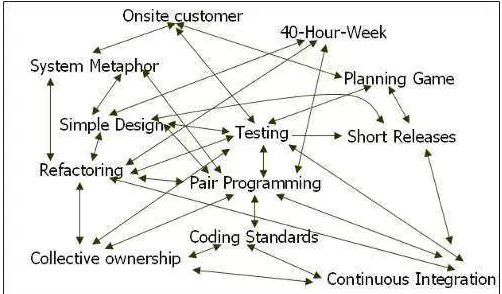
\includegraphics{beck.png}
\caption{XP practices \cite{beck_extreme_2000}. \label{XP}}
\end{figure}\\

Scheweigert et al had performed a study on Agile maturity models. Authors describes the status of the agile maturity models and conveys that the available maturity models are structured in a top level compilation \cite{schweigert_agile_2013}. In their article they provided an approach to analyze the agile maturity models in terms of extracting the content, mapping it to a reference models and finding the real agile maturity issues through synthesis \cite{schweigert_agile_2013}. They did not make any attempt in proposing a new maturity model within their research but they concluded that there is a need for scientific research in this particular topic i.e. Agile maturity models.

Demirors et al had made a study in assessing the agile maturity models to figure out the strengths and weakness of the agile maturity models/ frameworks. They have considered five maturity models available in the literature to know how sufficient these models can provide insights about an organization’s agile capability \cite{ozcan-top_assessment_2013}. They made an assessment on each maturity models with an assessment criterion in terms of fitness for purpose, completeness, definition of agile levels, objective and correctness through conducting a case study \cite{ozcan-top_assessment_2013}. They also figured out the strengths and weakness in each model and concluded that “there is a need to improve the maturity models for better guidance in agile process adoption, process improvement and process assessment" \cite{ozcan-top_assessment_2013}.

A wide range of investigation is going on agile since decades. Most of the articles \cite{melnik_perceptions_2002}, \cite{pikkarainen_deploying_2005}, \cite{sfetsos_empirical_2010} focuses only on the agile practices adoption and usage of the agile practices. For implementing these agile practices there needs to be a structured process and the agile maturity models helps the organizations to implement the agile practices in an order. Several maturity models have been published in the recent years which guides the organizations in a structured manner in implementing the agile practices for a better development process. But not all of these maturity models defined with particular order of implementing of the agile practices are empirically validated \cite{schweigert_agile_2013}, \cite{patel_agile_2009}, \cite{ozcan-top_assessment_2013}. This motivated authors to conduct this research.


\chapter{Research Method}
\section{Literature Review}
\noindent 
Hart defined literature review as “The use of ideas in the literature to justify the particular approach to the topic, the selection of methods, and demonstration that this research contributed something new” \cite{levy_systems_2006}. For conducting this literature review authors followed the guidelines provided by Levy and Dr. Rowley in the articles \cite{levy_systems_2006} and \cite{rowley_conducting_2004}. Literature review process is performed in three sequential steps Input, Processing and Output to know the existing knowledge on agile maturity models. Stages of the literature review process are performed in sequential steps to collect, know, comprehend, apply, analyze, synthesize and evaluation of the literature \cite{levy_systems_2006}, \cite{levy_towards_2006}. Initially input step comprises of gathering the manuscripts required for conducting the literature review. Next in the processing stage a detailed examination of the literature is carried out with identifying, summarizing, illustrating, comparing, connecting and generalizing the valid literature. Finally output step entails of documenting the results of the literature review by following the guidelines mentioned in the article  \cite{levy_systems_2006}, \cite{levy_towards_2006}. 

Literature review helps in finding out the existing body of knowledge related to the subject area. It also helps the authors to know what has done and what is needed to be done \cite{levy_systems_2006}. A literature review is conducted in this study to retrieve and understand different agile maturity models with the process involved in agile development. This resulted in gathering the agile maturity models and the order of practices implemented in each maturity model. This framed the basis for performing the research.

After getting finalized with the topic “Agile Maturity Models” the initial step to perform a background and related study, which has been performed and reported in the previous chapter 2 of the document. The next preliminary step is to perform a literature study to identify the work that has already been done in this field of research which enables the authors in providing insights about different agile maturity models. This provided the authors in gaining immense comprehensive knowledge about the software development involved with agile. Later on, literature searches are performed to extract all the published maturity models available in the scientific databases. The main aim of the literature review is to identify different maturity models with the identification of the order of practices recommended for the agile development. As mentioned earlier, the literature review is performed in three sequential steps. The steps are as follows:
\subsection{Input}
A literature review is conducted in this study for gathering agile maturity models from the existing literature, the objective of the literature review is to summarize the state of the art in this subject field [36]. Initially, authors framed the keywords as agile maturity models, agile maturity frameworks, agile assessment models and software process improvement for conducting the search. Using these keywords database search is performed in the scientific databases for retrieving the articles related to study. Initially, a search string was framed using Boolean AND/OR operations and is used in several scientific databases namely Google scholar, Engineering village, Scopus and BTH-Summon. According to the context and design of the databases the search string was modified to retrieve the article. The search string is presented in the Figure XXXX.
\begin{table}[h] 
\centering
\caption{Search string}
\label{search string}
\begin{tabular} {|p{9cm}|}
\hline
\textbf{Search string:} ((((agile maturity model) OR agile maturity framework) AND software process improvement) OR agile assessment model)\\
\hline
\end{tabular}
\end{table}
From the refined searches, all titles and abstracts were read thoroughly and the papers which describe about the agile maturity models were only considered. To find an effective literature it makes sense to look into conference papers, journals, and scientific articles [35], [37]. Hence, authors considered only the papers which were available in full text. To the best of the authors knowledge initially very less scientific articles were found which are related to the research topic. A start set of 8 research articles were considered.

Thereby reading the full text of the articles authors decided to perform forward literature and backward literature search as per the guidelines indicated in the article [35]. As the keyword search process is associated with the use of technology specific terms, keywords appears and disappear from the literature overtime. Therefore, backward and forward approaches are implemented for the ease of authors to follow the models, theories, theoretical constructs and research streams [35]. The forward and backward literature searches are performed to build a solid theoretical foundation for the study through extraction of additional essential information from the literature.

\textbf{Backward Literature search:} It is performed in three specific sub-steps backward reference search, backward author search and previously used keywords \cite{levy_systems_2006}. Backward reference search is performed through references of references as mentioned in the guidelines to possess a deeper knowledge of the evolution of agile maturity models \cite{levy_systems_2006}. Backward author search is referred as the search conducted based on the authors names. This helped in finding out the author's previous work and gathering the papers related to the field of study. The final step in this process is performed by using previously used keywords from the relevant papers This helped the authors in finding a total of 9 articles out of 75 that are related to the problem domain.

\textbf{Forward Literature search:} This is carried out in two ways: forward reference search and forward author search \cite{levy_systems_2006}. Forward reference search is performed through reviewing the articles that had cited the paper which further helped in finding the new literature. Forward author search is done by searching the papers related to the authors name. A total number of 36 papers were retrieved from this particular search but only 10 articles were relevant for this particular study.

The forward and backward literature search resulted in 33 numbers of articles but among these, the articles were only selected based on the inclusion criteria mentioned below with the relevance of the study \cite{kitchenham_systematic_2009}.
\begin{table}[h]
\centering
\caption{Articles information}
\label{articles}
\begin{tabular} {|p{6cm}|c|p{3cm}|}
\hline
\textbf{Research Articles} & \textbf{Database} & \textbf{No. of articles retrieved}\\ \hline
\cite{schweigert_agile_2013}, \cite{leppanen_comparative_2013}, \cite{fontana_maturing_2014}, \cite{ozcan-top_assessment_2013}, \cite{selleri_silva_reference_2014}, \cite{fontana_processes_2014}, \cite{fontana_progressive_2015}, \cite{qumer_framework_2008}, \cite{patel_agile_2009}, \cite{sidky_structured_2007}, \cite{benefield_seven_2010}, \cite{nawrocki_toward_2001}& Google Scholar & 12\\ \hline
\cite{pikkarainen_impact_2008}, \cite{pikkarainen_deploying_2005}, \cite{sfetsos_empirical_2010}, \cite{yin_scrum_2011}, \cite{ambler_agile_2009}, \cite{lui_road_2005}& Engineering Village & 6 \\ \hline
\end{tabular}
\end{table}

The table XXX shows the articles selected for conducting this particular study. The inclusion and exclusion criteria for this particular study is:\\
\textbf{Inclusion criteria:}
\begin{itemize}
\item	Papers discussing agile methodologies.
\item	Paper discussing agile practices.
\item	Papers related to the research problem domain (agile maturity model and agile maturity frameworks).
\item	Papers are selected only if it the text is in English.
\item	Articles available in full text.
\end{itemize}

\textbf{Exclusion criteria:}
\begin{itemize}
\item 	Papers older than 10 years  were excluded.
\item	Articles related to agile adoption in the non-software sector were excluded.
\item	Articles that are not peer reviewed were excluded.
\item Papers with a language other than English were excluded.
\item Duplicate studies are filtered and were eliminated.
\end{itemize}



\tikzstyle{startstop} = [ellipse, minimum size=1cm, text centered, draw=black, fill=white]
\tikzstyle{io} = [trapezium, trapezium left angle=70, trapezium right angle=110, minimum size=1cm, text centered, text width=3cm,draw=black, fill=white, inner sep=0pt]
\tikzstyle{process} = [rectangle, minimum size=1mm, text centered, text width=3cm,draw=black, fill=white]
\tikzstyle{decision} = [diamond, minimum size=1cm, text centered, text width=3cm, draw=black, fill=white, inner sep=0pt]
\tikzstyle{database} = [cylinder, minimum size=1cm, text centered, text width=3cm, draw=black, shape border rotate=90,aspect=0.25, fill=white]
\tikzstyle{line}= [draw, -latex']
\tikzstyle{arrow} = [thick,->,>=stealth]
\begin{figure} 

\centering
\begin{tikzpicture}[node distance=1.65cm]
\node (start) [startstop] {Start};
\node (pro1) [process, below of=start] {Area of Research};
\node (pro2) [process, below of=pro1] {Limiting Research area};
\node (in1) [io, below of=pro2] {Framing Keywords};
\node (pro3) [process, below of=in1] {Databases};
\node (datab) [database, right of=pro3, xshift=3.2cm] {Google scholar, Engineering village};
\node (pro4) [process, below of=pro3] {Conducting search};
\node (dec1) [decision, below of=pro4, yshift=-1.5cm] {Relevant Papers};
\node (pro5) [process, below of=dec1, yshift=-2cm] {Conducting forward and backward literature search};
\node (pro6) [process, below of=pro5, yshift=-1cm] {Filtering papers by inclusion and exclusion criteria};
\node (in2) [io, right of=pro6, xshift=3.2cm] {Final set of papers};
\node (stop) [startstop, right of=in2, xshift=2cm] {Stop};
\path [line] (start) -- (pro1);
\path [line] (pro1) -- (pro2);
\path [line] (pro2) -- (in1);
\path [line] (in1) -- (pro3);
\path [line] (pro3) -- (pro4);
\path [line] (pro4) -- (dec1);
\path [line] (pro3) -- (datab);
\path [line] (dec1) -- node [right, near start] {yes}(pro5);
\path [line] (pro5) -- (pro6);
\path [line] (pro6) -- (in2);
\path [line] (in2) -- (stop);
\path [line, rounded corners] (dec1) --++  (-4,0)node [above, near start] {no} |-(in1);

\end{tikzpicture}
\caption{Search strategy}
\end{figure}
Based on the above-mentioned inclusion and exclusion criteria each article is read thoroughly and only the relevant papers are selected. 9 different papers describe different agile maturity models. These 9 articles which describe different agile maturity models are synthesized and the process is described in detail in the further sections.
\subsection{Processing}
This processing stage involves in identifying and extracting the essential data which is presented in the article. Processing stage involved in analyzing each document through studying the full text of the document and making notes of each document. For conducting an effective literature study the guidelines provided by J Rowley and F Slack in the article “Conducting literature reviews” were followed \cite{rowley_conducting_2004}. This is carried out in five sequential steps: Scanning documents, making notes, structuring the literature review, writing the literature review and building the bibliography \cite{rowley_conducting_2004}.
\begin{itemize}
\item \textit{Scanning documents:} This is done to explore the literature which is relevant and reliable to the field of agile. The selected documents are carefully reviewed by both the authors and then they managed in grouping the documents with similar themes. This resulted in providing insights about the key themes related to agile maturity models which are essential for this study.
\item \textit{Making notes:} This involved with a detailed analysis and synthesis of the whole content of each article. Each article is studied thrice and all the essential information and data is noted through annotating and marking up the document. This information acts as backbone while answering the research question and so it was carefully reviewed.
\item \textit{Structuring the literature review:} This involved in identifying the key themes with the organization of concepts and documents together according to the actual research area. This helped in underlying the structure of different maturity models. A clear understanding of the maturity models with its set of agile practices is achieved through structuring the literature. Moreover, a defined purpose of the maturity models is gathered here.
\item \textit{Writing the literature:} An overview of each extracted maturity models is reported with a complete reference to that particular document. In this process of analysis, each maturity model with different maturity levels is defined with its set of different agile practices. This provided a summary of required literature for the research field.
\item \textit{Building the bibliography:} All the credits to the selected articles are given by building the bibliography as they contributed to a new research. A bibliography is a list of all the sources that refer to in the literature review \cite{rowley_conducting_2004}. 
\end{itemize}

Through achieving all these above mentioned five steps it is clear that the process involved with literature review is almost complete.
\subsection{Output}
The output of the literature review is presented with a clear academic style of writing with the logical structure of all extracted agile maturity models. All the nine agile maturity models included in this study are compared and presented in a single table which presents a logical structure of each maturity model. Adding an additional benefit this table can be used to compare the maturity models with one another. This document of the literature review also provides the set of agile practices defined in each maturity model with respect to maturity levels of that particular model. A comprehensive overview of each maturity model is documented after the complete analysis and synthesis of the model to uncover the interdependencies between the maturity levels. By performing these steps authors successfully managed in presenting a clear overview of the agile maturity models presented in the results chapter 4.
\section{Survey}
A survey is a strategy or design for an empirical study “to provide a quantitative description of some fraction of the population through collecting the data” \cite{punter_conducting_2003}. Surveys are generally conducted as a representation of current or past situations.

Survey is opted as a part of research method for this particular research as this study aims at knowing the implementation of agile maturity models with respect to agile practices in the current IT industries. A quantitative research approach is chosen for this research as the quantitative data promotes comparison and statistical analysis \cite{wohlin_empirical_2003}.

Experiments are not chosen for this research as they are concerned with limited scope and most often they run in a laboratory setting \cite{wohlin_empirical_2003}. So this type of approach for this research is not suitable. Moreover, experimentation objectives are to manipulate one or more variable and control all another variable at fixed levels \cite{wohlin_empirical_2003}. This kind of approach will not help in gathering the required data i.e. retrieving of agile methods and practices from the current industry. 

Whereas even case studies are also not suitable for this research because case studies are used for monitoring project, activities or assignment with an aim at tracking a specific attribute or establishing relationships between attributes \cite{wohlin_empirical_2003}. The aim of this research is not confined to a specific agile maturity model rather it involves several models hence, case study is not preferred in this case
Post-mortem analysis can be performed for retrieving the current agile practices adopted in the industry. But post mortem is conducted by looking at project documentation \cite{wohlin_empirical_2003}.  It is not possible to gather the project documentation from industry as it is confidential post mortem analysis is ignored and is out of authors minds. 

Implementation of agile methods in the current industry is vast and the survey has the ability to provide a large number of variables to evaluate. Moreover, the survey helps in collecting the data from a larger population from different geographic locations. Hence, survey questionnaire is used to achieve the objective of the RQ2.

Explorative surveys are used as a pre-study to investigate agile practices implemented in the current industry \cite{robson_real_2016}. A professional questionnaire is created and the data is collected through a sample of the population from all over the globe. The main purpose of the questionnaire is to identify the order of practices of agile maturity models implemented in the current industry and facilitate the authors in identifying and understand the differences and commonalities with both the theoretical study and the exploratory study.
\subsection{Rationale for survey}
The rationale behind conducting the survey through questionnaire is to answer the second research question (RQ2). Survey is adopted as a method to identify the order of practices of agile maturity models implemented in industry. Several agile practices were identified while performing the literature review. These set of agile practices were incorporated into the questionnaire. This questionnaire is designed in an inclusive way to gather the data required even for the third objective by following the guidelines provided in \cite{fink_survey_2003}. This way of design helped in identifying and understanding the benefits and limitations of the order of practices currently implemented in the industry. Furthermore, the questionnaire helped in understanding the differences and commonalities between the literature study and current industrial experience in relation to agile maturity models. The main aim of this questionnaire is to extract all possible information from the respondents related to the agile practices that are implemented in a particular order.

Survey is opted as an empirical research method for this particular study because the survey can be administrated quickly and easily. Moreover, to identify the practices and activities from the current industry from different geographical locations within a short period of time the authors felt that survey serves as the best option for them. As it helps in understanding the opinions of the software practitioners directly, involving wider population. Even from the respondent’s side, the questionnaires gives them an option to share their own personal experience regarding the agile software development process.
\subsection{Form of Data Collection}
After the completion of literature, a self-administrated online web-based survey is conducted using Sosci survey (www.soscisurvey.de). This served as instrument conducting survey. For collecting the data, the sosci survey is used as it is convenient for use and also for distribution of the questionnaire to the respondents. Sosci survey is a free professional software package embedded different essential features like programmable filters, programmable layout, implementation of HTML and several others. These several vital features contributed towards creating a professional survey. The feature of automation in collecting the data provided by Sosci benefited both the respondents and authors in collecting the data without encountering any problems. So this form of data collection also provided flexibility and convenience for analysis. Hence, it is chosen as a means for collecting the data.
\subsection{Population of the survey}
The population involved in this particular study are current software engineers involved in agile development projects. The survey is conducted with the involvement of all functional groups from the developed companies. Convenience sampling was used other than probability sampling technique as the population chosen for this study involves the nearest and most convenient persons who act as respondents [40]. Most of the contacts involved with the survey were supervisor and authors’ business contacts and so convenience sampling is adopted. For this survey, the experienced software practitioners are involved with the experience of agile development such as project managers, designers, developers, testers, analysts, etc. Respondents with agile experience and knowledge were only selected for answering the questionnaire to maintain the consistency in the quality of the responses, as this piece of valuable information is essential and crucial for further execution of the entire research. The respondents were contacted through email. With a superior request of the authors’ contacts, some of the respondents have forwarded the questionnaire to their colleagues who are experienced with the agile development to answer the questionnaire.

Authors also managed in publishing the survey in the social groups like LinkedIn groups, Yahoo groups and Google groups related to agile software development. The questionnaire is published only in the groups related to the agile software development which involved groups from India, Sweden, Scotland, Spain, Belgium, Finland and the United States. The respondents were contacted through a defined email containing the survey link with a brief description and objectives of the questionnaire, providing them with the necessary contact details for further inquiries. 
\subsection{Survey Design}
\noindent
The questionnaire is designed after the completion of the analysis of literature review by following the guidelines by A. Fink \cite{fink_how_2003}. The questionnaire is focused on the topics related to adoption of agile practices, its benefits, and limitations. The question for the questionnaire is developed in a systematic iterative process with a keen interest on understandability. The developed questions are evaluated by both the authors through discussions. Each question is mapped to the respective research question and analyzed how well the developed question is able to answer the research goals. The questionnaire consists of 11 close ended and 5 open ended questions to answer the RQ2 and RQ3. Not all questions involved in the questionnaire are similar to each other, the format of the questions varies accordingly. The close-ended questions contain multiple choice questions whereas open-ended questions are provided with the text fields in which the respondents are requested to share his/her own experience in their own words expecting that this could provide a clear response to that particular question.

The survey questionnaire consists of three web pages. For the reasons of conciseness in the document the whole questionnaire is not presented here but the complete questionnaires can be found in the appendix \ref{appendix A} and also it can be accessed online for a better professional experience when taking the survey. An overview of all the three webpages of the questionnaire is described below in separate sections.
\begin{itemize}
\item \textbf{Welcome Page:} In the first web page, a brief introduction about the survey is provided mentioning the non-disclosure statements of the respondent details. The contact details of the persons responsible for this particular questionnaire is included for any further inquiries.
\item \textbf{First Page:} In this page, the questionnaire starts with a question related to the adoption of agile practices. A list of 17 core agile practices are listed in the first question, correspondingly to each agile practice, a timeline (refer appendix A) is provided which is created using javascript. The timeline has a pointer to mark the adoption of practices with respect to the time frame. A clear description of each agile practice is provided adjacent to the agile practice in the information tag for the convenience of the respondents.  In the next part of the questionnaire, the respondents are requested to answer with reference to the agile practices adoption that they described in the previous question. Five open-ended questions are presented here which answers
\begin{itemize}
\item  The measures of success with agile adoption,
\item Limitations/ challenges faced during the implementing the agile practices,
\item Reasons for adopting the agile practice in that particular way of order and
\item Inquiries if any practice was terminated during the development process or not.
\end{itemize}
Within this page, the data related to the adoption of agile practices is gathered. At the end of this page, a comment section is provided with an open text field for the respondent to add any additional information if they want to.
\item \textbf{Second Page:} This second page is oriented with the research of this study including nine demographic questions. While entering to this page the respondent is requested to provide his/ her own background details regarding years of experience, roles, responsibilities and project characteristics. This page consists of 9 close-ended questions for the respondent to answer. These questions are related to the characteristics of their development teams, development type, industry domain and type of systems the respondent is experiencing or experienced previously. Also, the details of their distribution of team members are asked through a close ended question. This page completely focuses on retrieving the respondent’s own experience with the adoption of agile practices.
\item \textbf{Third Page:} And finally on the last page the respondent is optionally asked to add another experience. If the respondent does not want to add another experience, then he/she is asked to provide their contact details if they are interested in the survey results and for any further inquiries. Then the respondent is greeted with a vote of thanks for participating in the survey finally asking if they want to share anything else with us.
\end{itemize}
\subsection{Piloting Survey}
The questionnaire must be pre-tested before conducting the main survey to ensure whether the mentioned questions and inserted functionalities are functional, understandable and user-friendly or not. This helps the authors to find the difficulties faced by the respondents before conducting the main survey \cite{kelley_good_2003}. To conduct the pilot survey initially, the questionnaire is discussed and tested with the supervisor to detect any flaws in the questionnaire. With the feedback given by the supervisor additionally, a question was added to the questionnaire which is beneficial to our study. The test link of the questionnaire was finalized. As suggested by the Kate Kelly \cite{kelley_good_2003} the pilot survey is conducted.

Three respondents were selected and the link was forwarded to them with an invitation email to participate in the survey. The pilot survey is conducted with the three respondents where all the respondents are software practitioners related to agile software development from the reputed companies. All the three respondents are well experienced with the agile software development methodologies. After a detailed analysis of the feedback given by the three respondents authors came to notice that the slider functionality which is included to answer the 1st question in the questionnaire was not functioning smoothly, overall every respondent commented that the questionnaire content was professional. After conducting the pilot survey, the questionnaire is validated by adding the information about the use of slider functionality in detail. Moreover, several enhancements were made to the code for the smooth running of functionality. Thus, the pilot survey helped the authors to finalize the questionnaire and publish the survey under the guidance of the supervisor.
\subsection{Survey Execution}
The survey is sent to the respondents through emails.  With welcome note, a brief description of the survey and the estimated time to complete the survey is mentioned in the contents of the mail (refer appendix \ref{appendix A}). A log of all the respondents to whom the mail is distributed and the details of that particular respondent is maintained and updated frequently to avoid the reoccurrence of sending invitation mails to the same respondent again. The authors managed in publishing the survey link in the widely used social network websites namely LinkedIn, Yahoo groups and Google groups. The survey link is only posted in the frequently used groups related to agile methodologies. Above all the respective supervisor also contributed in gathering the responses.
\begin{figure}[h]
\centering
\label{Survey execution}
\begin{tikzpicture}[node distance=1.65cm]
\node (start) [startstop] {Start};
\node (pro1) [process, below of=start] {Define objectives of survey};
\node (pro2) [process, below of=pro1] {Planning the survey};
\node (pro3) [process, below of=pro2] {Population sampling};
\node (pro4) [process, below of=pro3] {Questionnaire design};
\node (dec1) [decision, below of=pro4, yshift=-1.5cm] {Validating questionnaire};
\node (pro5) [process, right of=dec1, xshift=3.5cm] {Publish the survey};
\path [line] (start) -- (pro1);
\path [line] (pro1) -- (pro2);
\path [line] (pro2) -- (pro3);
\path [line] (pro3) -- (pro4);
\path [line] (pro4) -- (dec1);
\path [line] (dec1) -- node [above, near start] {yes}(pro5);
\path [line, rounded corners] (dec1) --++  (-4,0)node [above, near start] {no} |-(pro4);

\end{tikzpicture}
\caption{Survey execution}
\end{figure}
\newpage
\section{Interviews}
The survey can be conducted through two possible ways that are either by sending a questionnaire or by interviewing people with the available target population \cite{wohlin_empirical_2003}. The primary means of gathering the qualitative and quantitative data are through interviews or questionnaires \cite{wohlin_empirical_2003}. Interviews were used to validate the derived order of agile practices and also the checklist developed for the ease of software practitioners which involves the implementation of recommended order of agile practices.

A checklist is developed after the completion of the analysis of the extracted data from literature, questionnaire and interviews. A recommended order of agile practices during software development process is proposed with a view to benefit the current software practitioners and also the checklist is validated through performing interviews. Interviews are held with the respondents who are highly experienced within the agile project development. After carefully selecting the interviewees a semi-structured approach is followed with specific open-ended questions to gather all the essential data required to validate the checklist. Since all of the contacts are author’s business contacts telephonic or video calling were adopted for executing the interviews.

Therefore, interviewers contributed towards assessing usability, usefulness and readiness of the checklist and helped authors in providing necessary enhancements to finalize the checklist. This framed checklist is believed by the authors that it helps the software practitioners while adopting the agile practices in an efficient way. The interviews protocol has been described in the figure \ref{protocol}.
\begin{figure}[h]
\centering

\begin{tikzpicture}[node distance=1.65cm]
\node (start) [startstop] {Start};
\node (pro1) [process, below of=start] {Define objectives of Interviews};
\node (pro2) [process, below of=pro1] {Planning the Interviews};
\node (pro3) [process, below of=pro2] {Designing Interview questionnaire};
\node (dec1) [decision, below of=pro3, yshift=-1.5cm] {Validating questionnaire};
\node (pro4) [process, right of=dec1, xshift=3.5cm] {Conducting the Interviews};
\path [line] (start) -- (pro1);
\path [line] (pro1) -- (pro2);
\path [line] (pro2) -- (pro3);
\path [line] (pro3) -- (dec1);
\path [line] (dec1) -- node [above, near start] {yes}(pro4);
\path [line, rounded corners] (dec1) --++  (-4,0)node [above, near start] {no} |-(pro3);

\end{tikzpicture}
\caption{Interview protocol}
\label{Interview protocol}
\end{figure}
\subsection{Rationale for Interviews}
The rationale for conducting the interviews is to validate the proposed order of agile practices which is developed for the ease of current software practitioners involved with the development of agile practices. The suitability, usability, usefulness, and completeness of the checklist is validated with the interviewers.
\subsection{Interview Questions}
The interview questions are framed with an aim to evaluate the proposed order of agile practices. The quality criteria used to evaluate this checklist is based on the following aspects
\begin{itemize}
\item	Readability and understandability of the checklist.
\item	Appropriateness of the checklist.
\item	Acceptability of the checklist.
\item	Applicability and suitability of the checklist.
\item	The complexity of the checklist.
\end{itemize}

Based on this criterion the questions for conducting the interview are framed. The interviews are conducted in a semi-structured approach. Semi-structure interviews are chosen as they contain open ended questions. “Open-ended responses are often elicited in organizational research to gather new information about an experience or topic, to explain or clarify quantitative findings, and to explore different dimensions of respondents’ experience” \cite{jackson_concept_2002}. The below mentioned table 3.1 is the framed interview questionnaire for conducting the interviews.
\begin{longtable}[H]{|p{1cm}|p{13cm}|}
\caption{Interview Questionnaire. \label{interview questionnaire}}\\\hline
\textbf{S.No} & \textbf{Interview Questions}\\ \hline
1. & Do you find any issues or difficulties with the proposed order of practices for better enhanced development process especially while implementing agile methodologies? If yes, please specify them.\begin{enumerate}
\item Face-to-face meeting
\item Self-organizing cross functional teams
\item On-site customer.
\item	Time boxing/ Sprint/ Iteration.
\item Planning game/ Sprint planning meeting.
\item	Simple design.
\item	Tracking progress.
\item	Coding standards.
\item	Iteration Reviews/ Retrospectives.
\item	Daily standup meetings.
\item	Continuous Integration.
\item	Short Iterations and Frequent releases.
\item	Metaphors and stories.
\item	Collective ownership.
\item	Refactoring.
\item	TDD.
\item	Pair programming.
\end{enumerate}\\ \hline
2. & Did you find any difficulties in understanding the language with respect to the attached checklist?\\ \hline
3. & Are the phrases and terminology used in the checklist are clearly understandable and familiar to the software engineering practitioners?\\ \hline
4. & Are there any benefits/ challenges which you can report if the practices are implemented in the above mentioned order?\\ \hline
5. & Do you find this checklist usable and suitable for implementing the agile practices? \\ \hline
6. & Are there any valuable suggestions/ comments which you can suggest to enhance this checklist for the use of practitioners?\\ \hline
\end{longtable}

\subsection{Interview Execution}
Interviews are conducted to validate the order of agile practices obtained from the results of the questionnaire. The prepared questionnaire for the interviews is documented and a brief description of objectives for the interview is sent to the respondents through email (refer appendix \ref{appendix C}). After sending an email an appointment is fixed based on the availability of the respondent. Interviews are conducted according to the convenience of the respondent either through telephone or video calling.  

\section{Mapping of Research Questions to Research Methodology}
For answering each research question several sequential steps are followed as described in the following table with the mapping of the research methodology to the respective research questions.
\begin{longtable}[h]{|c|p{5cm}|p{4cm}|}

\caption{Mapping Research Questions to Research Methodology. \label{mapping}}\\
\hline
\textbf{Research Questions} & \textbf{Research Steps} & \textbf{Research Methodology}\\ \hline
1. RQ1 &
1.1. Identifying the agile maturity models present in the literature. \newline 1.2. Identifying the order of practices from the each maturity model.& Literature review\\ \hline
2. RQ2 & 2.1. Identifying the order of practices implemented in the industry. & Survey\\ \hline
3. RQ3 & 3.1. Identifying the benefits and limitations in a certain order.\newline 3.2. Differences and commonalities were gathered by comparing and analyzing both the results of literature review and survey. & Literature Review , \newline Qualitative Data Analysis\\ \hline
4. RQ4 & 4.1.	 Develop a new checklist with the order of practices.\newline
4.2.	Validating the checklist through interviews. \newline
4.3.	Final checklist is proposed.\newline & Quantitative Data Analysis, \newline Interviews \\ \hline

\end{longtable}
\section{Data Analysis}
\subsection{Narrative Analysis}
Narrative analysis is a comprehensive narrative synthesis of previously published information \cite{green_writing_2006}. So the extracted data from the articles found from the database search and through forward and backward search is subjectively analyzed through performing the narrative analysis. Both the qualitative and quantitative research can be analyzed through narrative analysis \cite{petticrew_testing_2009}. Narrative overviews, also known as unsystematic narrative reviews provide findings in a condensed format that typically summarize the whole content of each article. This utilization of narrative overviews provided a clear insight about each maturity model depicting the maturity levels with the set of agile practices within each level. The data extracted from the literature was analyzed using narrative analysis for achieving the O1 and also for answering the RQ1.
\subsection{Statistical Analysis}
For analyzing the extracted data from the questionnaire authors performed statistical analysis, as the obtained data is based on quantitative variables \cite{sapsford_data_2006}. With the use of statistical methods, the quantitative data is analyzed to retrieve the order of agile practices implemented in the IT sector.
\subsubsection{Friedman Test}
A statistical analysis was performed to retrieve the most used practices that are reported by the respondents with the use of Freidman tests. “Nonparametric tests, based on ranks, are alternatives to parametric statistics for testing a hypothesis about differences for variables measured on an ordinal scale” \cite{sheldon_use_1996}, \cite{robson_real_2016}. Friedman developed a procedure called method of ranks to test hypothesis related to ordinal scale \cite{sheldon_use_1996}. Mean ranks are calculated with the standard deviation variance of each variable. Mean ranks are calculated for all the agile practices included in the questionnaire. Through conducting Friedman test it helps in discovering the most frequently used agile practices.  Based on the mean ranks, the most implemented agile practices in the industry are extracted from the collected quantitative data.

The computational formula for the Friedman test is \cite{sheldon_use_1996}.

\[\chi^2_r=\frac{12}{Nk(K+1)}\sum_{j=1}^{k=1} R^2_j- 3N(k+1)\]






\[S1(\delta, \epsilon, A, B)= \frac{LCSS_{\delta,\epsilon}(A,B)} {\text{min}(n,m)}\]


\begin{equation}
LCSS_{\delta, \epsilon} (A, B)=
\left \{ \begin{array} {l p{4cm}}
	0,  & \text{if A or B is empty}
	\\
	1+ LCSS_{\delta, \epsilon} (Head(A), Head(B)), 
	 & \text{if} |\ a_{x, n}-b_{x,m}|\ < \epsilon  \text{and} |\ a_{y,n}-b_{y,m}|\ < \epsilon  \text{and} |\ n-m |\ \leq \delta
	\\
	\text{max} (Head(A), B), LCSS_{\delta, \epsilon}(A, Head(B))), & \text{otherwise}
	\end{array} \right
\end{equation}


















\begin{flushleft}
where\\
K= Number of ranked observations or measurements\\
N= Number of subjects (rows)\\
RJ= Sum of ranked scores in each column\\
The numbers 12 and 3 are constants and the test statistics\\

\end{flushleft}
The number 12 and 3 are constants and the test statistic $\chi^2_r$ is distributed according to the usual $\chi^2$ distribution with $k-1$ degree of freedom when the ranking are random. After getting the $\chi_r^2$ value it should be compared with the chi-square distribution chart. The  obtained $\chi_r^2$ value makes a decision to approve or disapprove the null hypothesis. Before this, by following the chi-square distribution table with an alpha level of 0.05 and the degree of freedom, a critical value is obtained. That means that if the $\chi_r^2$ value is greater than the obtained critical value then the null hypothesis is rejected. The degree of freedom is calculated by using a formula
\[df=k-1\]

Where $k$ for this research is number of agile practices included in the observations. The null hypothesis is rejected through comparing the critical values of chi-square distribution as shown in the table \ref{chi-square}.

\begin{longtable}[h]{|p{4cm}|p{4cm}|p{4cm}|}
\caption{Critical values of the Chi-square distribution.\label{chi-square}}\\
\hline
\textbf{$df$} & \textbf{$\chi^{2*}_.05$} & \textbf{$\chi^{2*}_.01$}\\ \hline
1&	3.841&	6.635\\ \hline
2&	5.991&	9.210\\ \hline
3&	7.815&	11.345\\ \hline
4&	9.488&	13.277\\ \hline
5&	11.070&	15.086\\ \hline
6&	12.592& 16.812\\ \hline
7&	14.067&	18.475\\ \hline
8&	15.507&	20.090\\ \hline
9&	16.919&	21.666\\ \hline
10&	18.307&	23.209\\ \hline
11&	19.675&	24.725\\ \hline
12&	21.026&	26.217\\ \hline
13&	22.362&	27.688\\ \hline
14&	23.485&	29.141\\ \hline
15&	24.996&	30.578\\ \hline
16&	26.296&	32.000\\ \hline
17&	27.587&	33.409\\ \hline
18&	28.869&	34.805\\ \hline
19&	30.144&	36.191\\ \hline
20&	31.410&	37.566\\ \hline
21&32.671&	38.932\\ \hline
22&	33.924&	40.289\\ \hline
23&	35.172&	41.638\\ \hline
24&	36.415&	42.980\\ \hline
25&	37.652&	44.314\\ \hline
26&	38.885&	45.642\\ \hline
27&	40.113&	46.963\\ \hline
28&	41.337&	48.278\\ \hline
29&	42.557&	49.588\\ \hline
30&	43.773&	50.892\\ \hline

\end{longtable}
\subsection{Comparative Analysis}
Without comparisons, there is no complete fulfillment to any research. Qualitative data is useful in supplementing and illustrating the data obtained from the survey \cite{robson_real_2016}. The qualitative comparative analysis supports with logical conclusions to the data set. There are many ways to conduct a comparative analysis through application of different logical techniques \cite{robson_real_2016}. Comparative analysis for this study is conducted to discover the commonalities and differences between the results of survey and literature review to uncover the benefits and limitations of implementing the agile practices. This type of analysis is also carried out for further discussions and helped authors in framing new findings to the research.
\subsection{Thematic Analysis}
Thematic analysis is a method used to analyze the qualitative data and to report the patterns (themes) in the collected data \cite{lacey_qualitative_2001}, \cite{wohlin_towards_2015}. Thematic analysis is chosen to analyze the qualitative part of the study and it is one of the commonly used methods for analysis in empirical research. Authors performed thematic analysis in sequential steps as suggested in the article \cite{lacey_qualitative_2001} and the steps are as follows
\begin{itemize}
\item \textbf{Transcribing:} The data collected is transcribed into a document in written format.
\item \textbf{Organizing data:} The transcribed data is organized accordingly to analyze it for easy retrieval of the data.
\item \textbf{	Familiarization with data:} The data which organized are read carefully for a clear understanding of the data collected.
\item \textbf{Coding:} Identifying the code is done by manually and carefully examining the data collected. A tag is assigned to each code for easy identification.
\item \textbf{Generating themes:} After identifying the codes then the codes are categorized into themes. Later themes are labeled with a name for reporting the results.
\end{itemize}
\subsection{Alternate analysis method}
For both the quantitative and qualitative data there are several options to analyze the data. One of the suitable options to analyze the data would be grounded theory. According to Polit and Beck \cite{hussein_using_2014} “a generalization is an act of reasoning that involves drawing broad conclusions from particular instances” and they also espoused that knowledge is not gathered by testing a new theory but knowledge grows through confirmation \cite{hussein_using_2014}. There are several limitations with the grounded theory and in \cite{hussein_using_2014} reports that generalization is limited through grounded theory for the interpretation and analysis of data. Also, while performing grounded theory any prior consideration regarding the data shouldn’t be made whereas for this particular research the extracted data is certain for its analysis and purpose. Hence grounded theory is not appropriate for this research.





\chapter{Results}
\section{Results from Literature Review}
This paper has unique characteristics from the currently available literature based on agile methodologies. This document provides a detail comprehensive knowledge on nine agile maturity models published in recent years. Owing to the limited available resources on agile maturity models authors performed in-depth analysis and synthesis for presenting these nine agile maturity models. With a keen eye on the data extraction process, the overview of each maturity model is constructed based on the published structure of each maturity model with its defined set of agile practices. One after the other the overview of each maturity model is presented below. For each maturity model a respective ID is assigned for convenience in addressing the maturity model and is represented in the table \ref{ID}.
\begin{longtable}[h] {|p{2cm}|p{3cm}|p{2.8cm}|p{2.5cm}|p{2cm}|}

\caption{Assigned ID's for identified agile maturity models. \label{ID} }\\
\hline
\textbf{Model ID} & \textbf{Paper Title} & \textbf{Model name} & \textbf{Author Name}& \textbf{Reference}\\ \hline
M1& Agile Maturity Model (AMM): A software process
improvement framework for Agile Software Development 
practices. & Agile Maturity Model (AMM)& Chetankumar Patel and Muthu Ramachandran& \cite{patel_agile_2009}\\ \hline
M2& A Framework to support the evaluation, adoption
and improvement of agile methods in practices & Agile Adoption and Improvement Model (AAIM) & A. Qumber and B. Henderson & \cite{qumer_framework_2008}\\ \hline
M3 & A Reference Model for Agile Quality Assurance: Combining Agile methodologies and Maturity Models & Agile Quality Assurance-Reference Model (Agile QA-RM) & Fernando Selleri Silva and Et.al & \cite{selleri_silva_reference_2014}\\ \hline
M4 & A Structured approach to Adopting Agile Practices:
The Agile Adoption framework & Sidky Agile Measurement Index (SAMI) & Ahmed Sidky & \cite{sidky_structured_2007}\\ \hline
M5 & Seven Dimensions of Agile Maturity in the Global Enterprise: A Case Study & Benfield's Model & Robert Benfield & \cite{benefield_seven_2010}\\ \hline
M6 & Scrum Maturity Model& Scrum Maturity Model&Alexandre Paulo Guo Yin& \cite{yin_scrum_2011}\\ \hline
M7 & The Agile Scaling Model (ASM): Adapting Agile methods for complex environments& Agile Scaling Model (ASM) & Scott W. Ambler& \cite{ambler_agile_2009}\\ \hline
M8 & A Road Map for Implementing XP & XP Model& Kim Man Lui and Keith C.C. Chan& \cite{lui_road_2005}\\ \hline
M9& Towards Maturity Model for extreme Programming (XP) & The eXtreme Programming Maturity Model (XPMM) & Jerzy Nawrocki, Bartosz Walter, Adam Wojciechowski.& \cite{nawrocki_toward_2001}\\ \hline
\end{longtable}
\subsection{M1: Agile Maturity Model (AMM)}
This model was developed by Patel, et.al. focusing on adaptability, sustainability and software maturity model \cite{patel_agile_2009}. This AMM is designed with the intention to improve, enhance and boost up the agile software development methodology through increasing the customer satisfaction, software quality, etc. Based on the agile principles and practices this model is designed with five maturity levels. From initial to ad-hoc level predefined practices for each level is defined to enhance the development process. With a focus on the research, the activity and set of practices have been retrieved from each level as described below.
\begin{enumerate}
\item \textbf{Initial:} The first level is named as “Initial” where there are no predefined goals or activities due to instability in the process of development.
\item \textbf{Explored:} The second level is defined as “Explored”. The focal point of this level is on planning, requirements engineering, and customer satisfaction. At this level to give a good kick-start to the project an effective project planning, story card is driven development and involvement of the customer during the project for changes in requirements is followed in order to improve efficiency from the problems related to planning and requirements engineering.
\item \textbf{Defined:} At “Defined” level 3 the main focus is on the practices related to customer relationship management (CRM), frequent deliveries, pair programming, communication, coding, testing and quality of software\cite{patel_agile_2009}. The practices involved in this level are collective ownership, refactoring, frequent releases, coding standards, pair programming, and TDD.
\item \textbf{Improved:} At level 4 the maturity of the organizations is improved when comparing to previous levels hence it is named as Improved. At this point of time, the organizations are in a position to measure and control the software development process or practices and product quality with a main focus on the project management, working hours, risk assessment, self-organizing teams and problems related to the development team \cite{patel_agile_2009}.
\item \textbf{Sustained:} Level 5 the highest level of this particular maturity model named as sustained mature level. At this level companies focus on performance management and defect prevention practices through quantitative feedback from the process and from testing innovative ideas and technologies \cite{patel_agile_2009}.
\end{enumerate}
\begin{table}[h]
\centering
\caption{My caption}
\label{my-label}
\begin{tabular}{|c|p{1.5cm}|p{2cm}|p{2.1cm}|p{2cm}|p{2cm}|}
\hline
\textbf{Model ID} & \multicolumn{5}{l|}{\textbf{Maturity levels}}        \\ \hline
                  & \textbf{Level-1: Initial} & \textbf{Level-2: Explored}                                                                                                               & \textbf{Level-3: Defined}                                                                                                                                                                                                 & \textbf{Level-4: Improved}                                                                                                                     & \textbf{Level-5: Sustained}                                                                                            \\ \hline
M1                &                  & \begin{tabular}[c]{@{}l@{}}1. Planning \\game\\ 2. On-site\\ customer\\ 3. Stories\\ (Story card \\ driven \\development)\end{tabular} & \begin{tabular}[c]{@{}l@{}}1. Collectiv-\\e ownership\\ 2. Refactor-\\ing\\ 3. Short\\ Iterations \&\\ Frequent \\releases\\ 4. Coding\\ standards\\ 5. Pair Pro-\\gramming\\ 6. Test \\Driven \\ Development \\(TDD).\end{tabular} & \begin{tabular}[c]{@{}l@{}}1. Tracking\\ progress\\ 2. Time \\boxing\\ 3. Self-\\organizing \\teams\\ 4. Contin-\\uous \\Integration\end{tabular} & \begin{tabular}[c]{@{}l@{}}1. Time \\boxing\\ 2. Contin-\\uous \\Integration\\ 3. Story \\card with\\ TDD\end{tabular} \\ \hline
\end{tabular}
\end{table}

After a detailed synthesis in this particular maturity model it is identified that the order of practices in this model helps the team in identifying and improving problems related to CRM, frequent releases, coding standards and testing \cite{patel_agile_2009}. But in especially at level 3 implementation of few essential practices like structured risk management, code optimization, and solving problems occurred due to the team is missing. While gaining maturity it aims at self-organizing teams and improving the efficiency of project management, maintaining the sustainable pace to accomplish the project. The structure of this maturity model is relevant to the CMMI levels with the implementation of various agile practices. Since implementing the CMMI model for software process improvement is still a challenging issue for organizations following agile methods. Thus, authors have developed this framework on agile development process with a focus on adaptability, suitability and process improvement. 
\subsection{M2: Agile Adoption and Improvement Model (AAIM)}
An Agile Adoption and Improvement Model (AAIM) was developed by A. Qumber and B. Henderson and published as an article. A framework to support the evaluation, adoption and improvement of agile methods in practice, they summarized agile method as \cite{qumer_framework_2008}.
\begin{center}
\textit{Agile method = f (agility, abstraction, people, process, product, tools, knowledge, governance)}
\end{center}
In this agile adoption and improvement model authors have categorized the model into three agile blocks namely agile block: prompt, agile block: crux and agile block: apex. Where each level implements several agile practices throughout the software development process.
\begin{enumerate}
\item \textbf{Prompt:} It involves only one level called agile infancy the agile practices implemented in this level are iteration planning, TDD, and on-site customer \cite{qumer_framework_2008}. Thereby this level is mentioned as Agile infancy.
\item \textbf{Crux:} While entering into the second block referred as crux it consists of three sub-levels. The first level is called as agile initial, it enables in establishing good communication and collaboration with both the customers and relevant stakeholders \cite{qumer_framework_2008}. Whereas the next level termed as agile realization emphasizes on minimal documentation with the encouragement of verbal or face-to-face communication and tools. The final level of the crux is labeled as agile value aims at establishing the agile practices with a focus on development tools and practices \cite{qumer_framework_2008}.
\item \textbf{Apex:} The final block Apex contains two levels agile smart and agile process it aims at reducing cost while improving the production quality \cite{qumer_framework_2008}. Agile smart involves a smart learning curve of software development, software process, software quality and new tools. The last level of this maturity model focuses on the establishment of the lean production environment to keep the process agile thus it is named as agile process \cite{qumer_framework_2008}.
\end{enumerate}

\begin{longtable}[h]{|l|p{2cm}|p{2cm}|p{2cm}|p{2cm}|p{2cm}|}
\caption{My caption}
\label{my-label}\\
\hline
\textbf{Model ID} & \multicolumn{5}{l|}{\textbf{Maturity Levels}}                                                                                                                                                                                                                                                                                                                                                        \\ \hline
                  & \textbf{Level-1: Agile Infancy}                                                                                          & \textbf{Level-2: Agile Intial}                                                                    & \textbf{Level-3: Agile Realization} & \textbf{Level-4: Agile Value} & \textbf{\begin{tabular}[c]{@{}l@{}}Level-5: \\Agile\\smart\\ Level-6:\\ Agile\\ progress\end{tabular}} \\ \hline
M2                & \begin{tabular}[c]{@{}l@{}}1. Iteration \\planning\\ 2. Test-\\Driven \\Developm\\ent (TDD)\\ 3. On-site \\customer\end{tabular} & \begin{tabular}[c]{@{}l@{}}1. face-to-\\face\\ communic-\\ation\\ 2. Daily\\ stand up \\meeting\end{tabular} & 1. minimal documentation            & 1. Self-organizing teams      &                                                                                                 \\ \hline

\end{longtable}

The analysis on this maturity model tells that this a method is an independent model which guides the agile practitioners. This AAIM model helps in measuring and assessing quantitatively with the degree of software agility through providing a systematic road map for implementing the agile practices to the software development environment \cite{qumer_framework_2008}. This model provides a communication cooperation protocol in order to increase the efficiency of communication reducing the documentation. It comprises of mixed agile and traditional incremental development practices like product backlog, project planning, pair programming, product architecture, design, TDD, Coding, testing, and retrospective. The agile adoption and improvement model (AAIM) is validated empirically with one medium and one large sized organization in the area of embedded systems, network solutions, e-commerce systems, print solutions and multimedia production \cite{qumer_framework_2008}.
\subsection{M3: Agile Quality Assurance-Reference Model (Agile QA-RM)}
With several authors F. Selleri Silva, et.al combined agile methodologies and maturity models framed an Agile Quality Assurance- Reference Model (Agile QA-RM) \cite{selleri_silva_reference_2014}. This model consists of five maturity levels with 18 process areas similar to CMMI and MPS.BR structure. An overview of each level with defined agile practices is reported below with reference to the article \cite{selleri_silva_reference_2014}.
\begin{itemize}
\item \textbf{Informal QA:} Initially, practices related to quality assurance (QA) like audits, monitoring and review are implemented in the level 1 i.e. Informal QA.
\item \textbf{Managed QA:} At this level activity related to quality such as requirement analysis, testing and development are planned. This level is aligned with specific practices related to Quality Assurance Planning (QAP), Team Assistance (TEA), Processes Assessment (PCA), Non-Compliance Management (NCM), Product Assessment (PDA) and customer Satisfaction (CSA) are carried out to increase the satisfaction along the sprints \cite{selleri_silva_reference_2014}. The practices implemented at this level are planning game, on-site customer, daily meetings, coding standards, pair programming, iterations and sprint review meetings.
\item \textbf{Defined QA:} The next level is Defined QA which includes the process areas and generic practices of PPQA namely Organizational Quality Assurance (OQA), Knowledge Management (KMW), Lesson Learned Management (LLM), Integration Management (ITM), Quality Assurance Quality (QAQ), Cost Analysis (CTA) and Risk Analysis (RKA). The practices implemented at this level are self-organizing teams, retrospectives, face-to-face communication, continuous integration, metaphor, sprint planning meeting and daily standup meetings.
\item \textbf{Measure QA:} It comprises of application metrics responsible for enhancing the quality and development process or the product. It aims at Quality Assurance Measurement (QAM), Self-organization and Sustainability (SDS), overloads, schedule delays and costs increase. Practices like TDD, pair programming, self-organizing teams, and collective ownership are implemented at this level.
\item \textbf{Optimized QA:} The level 5 aims at optimizing the process. In this level, the process areas deal with defect prevention (DFP) and Decision-Making Support (DMS) in a proactive way to minimize noncompliance and support in decision-making \cite{selleri_silva_reference_2014}.
\end{itemize}

\begin{longtable}[h]{|c|p{1.5cm}|p{2cm}|p{2.2cm}|p{2.2cm}|p{2cm}|}
\hline
\centering

\textbf{Model ID} & \multicolumn{5}{l|}{\textbf{Maturity Levels}}                                                                                                                                                                                                                                                                                                                                                                                                                                                                                                                                                                                                                                                         \\ \hline
                  & \textbf{Level-1: Informal QA} & \textbf{Level-2: Managed QA}                                                                                                                                                             & \textbf{Level-3: Defined QA}                                                                                                                                                                                                       & \textbf{Level-4: Measure QA}                                                                                                                        & \textbf{Level-5: Optimized QA}                                                  \\ \hline
M3                &                               & \begin{tabular}[c]{@{}l@{}}1. Planning \\game\\ 2. On-site \\customer\\ 3. Daily \\meetings\\ 4. Coding \\standards\\ 5. Pair \\programm-\\ing\\ 6.Iterations\\ 7. Sprint \\review \\meeting\end{tabular} & \begin{tabular}[c]{@{}l@{}}1. Self-org-\\anizing \\teams\\ 2. Retrosp-\\ectives\\ 3. Face-to-\\face \\communic-\\ations\\ 4. Contin-\\uous \\integra-\\tion\\ 5. Metaphor\\ 6. Sprint \\planning \\meeting\\ 7. Daily \\meeting\\ 8. Retrosp-\\ective\end{tabular} & \begin{tabular}[c]{@{}l@{}}1.TDD\\ 2. Pair \\programming\\ 3. Self-\\organizing \\teams\\ 4. Collective \\ownership\end{tabular} & \begin{tabular}[c]{@{}l@{}}1. On-site \\customer\\ 2. Daily \\meetings\end{tabular} \\ \hline
\end{longtable}

An analysis of this maturity model showed similarities with Process and Product Quality Assurance (PPQ) with the CMMI. This model complies with CMMI and MPS.BR \cite{selleri_silva_reference_2014}. This model is not yet evaluated but is expected to evaluate with a set of Brazilian companies.
\subsection{M4: Sidky Agile Measurement Index (SAMI)}
Sidky published an Agile Adoption Framework in his thesis “Sidky Agile Measurement Index” \cite{sidky_structured_2007}. This Sidky Agile Measurement Index is described in 5 stage process which acts as a guide to the organization for software development process. Sidky has made an excellent attempt in relating the agile levels with the agile practices based on the agile principles. The set of practices listed with respect to each level is described below with complete reference of the article \cite{sidky_structured_2007}.
\begin{enumerate}
\item \textbf{Collaborative:} This level aims at intensifying the communication and collaboration in the software development process. The implementation of a set of agile practices in this level are retrospectives, planning game, self-organizing teams, coding standards, knowledge sharing, and on-site customer \cite{sidky_structured_2007}.
\item \textbf{Evolutionary:} The objective of this level is to enhance in collaborative work and delivering the software frequently. The set of practices involved at this level are short iteration, continuous delivery or frequent releases, sprint planning, tracking progress, simple design, customer contract reflective of evolutionary development \cite{sidky_structured_2007}.
\item \textbf{Effectiveness:} In this level, since the organization have already achieved effective communication and collaboration with frequent deliveries in the development process. The next objective at this level is to increase the efficiency and effectiveness of the development process \cite{sidky_structured_2007}. Hence, this level is named as Effective with the adoption of several agile practices. The set of practices involved are risk driven iterations, product backlogs, metaphors, self-organizing teams, frequent face-to-face communication, continuous integration, refactoring, and unit test.
\item \textbf{Adaptive:} This level helps in adopting practices that help in stabilizing and automate the software development process \cite{sidky_structured_2007}. This level the organization gather feedback from the customer to measure the correctness of the software product. Essential practices like on-site customer, iterative development, continuous customer satisfaction, frequent releases, adaptive planning, daily standup meeting, agile documentation, user stories and on-site customer \cite{sidky_structured_2007}.
\item \textbf{Encompassing:} In this level organizations accept the changes in the development process and maintain the agile nature. Seven essentials practices are implemented which ensure the highest level of maturity for the organizations through project estimation, low process ceremony, planning game, implementation of TDD, pair programming in small teams, frequent face-to-face \cite{sidky_structured_2007}.
\end{enumerate}


\begin{longtable}[h] {|c|p{2cm}|p{2cm}|p{2cm}|p{2cm}|p{2.2cm}|}
\caption{My caption}
\label{my-label}\\
\hline
\textbf{Model ID} & \multicolumn{5}{l|}{\textbf{Maturity Levels}}                                                                                                                                                                                                                                                                                                                                                                                                                                                                                                                                                                                                                                                                                                                                                                                                                                                                                                                                                                                                                                                                                                                                                                                                      \\ \hline
                  & \textbf{Level-1: Collaborative}                                                                                                                                                                                       & \textbf{Level-2: Evolutionary}                                                                                                                                                                                                                   & \textbf{Level-3: Effective}                                                                                                                                                                                                                                          & \textbf{Level-4: Adaptive}                                                                                                                                                                                                                                            & \textbf{Level-5: Encompassing}                                                                                                                                                                                           \\ \hline
M4                & \begin{tabular}[c]{@{}l@{}}1. Planning \\ game\\ 2. Self-\\ organizing \\and cross \\functional \\teams\\ 3. coding \\ standards\\ 4. Knowle-\\dge sharing \\ tools\\ 5. On-site \\customer\\ 6. Retrosp-\\ ectives\end{tabular} & \begin{tabular}[c]{@{}l@{}}1. Sprint \\planning\\ 2. Tracking \\iteration \\progress\\ 3. Short \\iteration \\ 4. Continu-\\ous delivery \\or frequent \\releases\\ 5. Simple \\Design\\ 6. Customer \\contract \\reflective of \\evolutionary \\development\end{tabular} & \begin{tabular}[c]{@{}l@{}}1. Risk dri-\\ven iterati-\\ons\\ 2. Product \\backlogs\\ 3. Metaph-\\ors\\ 4. Self-\\organizing \\teams\\ 5. Frequent \\ face-to-face \\communica-\\tions\\ 6. Continu-\\ous integra-\\tion\\ 7. Continu-\\ous improv-\\ement \\(refactoring)\\ 8. Unit tests\end{tabular} & \begin{tabular}[c]{@{}l@{}}1. On-site \\customer\\ 2. Iterations\\ 3. Continu-\\ous \\customer \\satisfaction \\feedback\\ 4. Frequent \\releases\\ 5. Adaptive \\planning\\ 6. Daily \\standup \\meetings\\ 7. Agile \\document-\\ation\\ 8. User \\stories\\ 9. On-site \\customer\end{tabular} & \begin{tabular}[c]{@{}l@{}}1. Low pro-\\cess \\ceremony \\ 2. Planning \\game\\ 3. Test \\driven \\development \\ 4. Pair \\programming\\ 5. Frequent \\face-to-face \\interaction \\between \\developers \\and users \\(collocated)\end{tabular} \\ \hline
\end{longtable}

Sidky proposed an Agile Adoption Framework consists of two components: Agile Measurement Index and 4-stage process. The Sidky Agile Measurement Index helps the organizations in measuring the agile potential. The 4-stage process helps the organizations in avoiding the conduct of unnecessary activities. This process is structured into four stages namely \cite{sidky_structured_2007}.
\begin{center}
\begin{enumerate}
\item Identifying Discontinuing Factors
\item Project Level Assessment
\item Organizational Readiness Assessment
\item Reconciliation
\end{enumerate}
\end{center}
Through framing a questionnaire with a total of 28 participants the goodness and effectiveness of the framework are validated.
\subsection{M5: Benfield's Model}
Benfield identified seven dimensions that are inconsistent to many of the teams. He published a new framework in the article “Seven Dimensions of Agile Maturity in the Global Enterprise: A Case Study” and named it as Benfield’s model \cite{benefield_seven_2010}. In this article, the author has considered seven dimensions to define the practices for each maturity level. The seven dimension are automated regression testing, code quality metrics, automated deployment and back out, automated builds and configuration management best practices, interlocked and interface integration testing, TDD, performance, and scalability testing. The five maturity levels which were defined based on the seven dimensions and also influenced by the CMMI, they are named as.
\begin{enumerate}


\item \textbf{Emergent Engineering Best practices:} This is the first level of the maturity model and the practices involved in this are unit testing, code reviews, repeatable builds, configuration management, code quality, and TDD. These are the practices implemented, valued and practiced by the team \cite{benefield_seven_2010}.
\item \textbf{Continuous practices at component level:} The level 2 is a repeatable rhythm of level 1. A deep understanding of previously introduced practices is made with the implementation of the practices. Reusable automation, interface testing, scalable testing is typically introduced. The unit harness is introduced with the implementation of the TDD in the implementation phase. The other practices implement at this level are user stories, metaphors, and tracking progress. The operation of previously introduced practices named this level as continuous practices at component level \cite{benefield_seven_2010}.
\item \textbf{Cross Component Continuous Integration:} This level focus on the robustness between a component with a flow through regular synchronized build/ test cycles across interface boundaries \cite{benefield_seven_2010}. Here the teams are aiming for a better synchronize work in order to improve the level of maturity and automation. The practices involved at this level are continuous integration, collaborative teams.
\item \textbf{Cross Journey Continuous Integration:} It composes of more sophisticated injection test harness and instrumentation This level exhibits within XP teams and ever shrinking end to end test cycles are implemented to increase the user experience and quality of the product \cite{benefield_seven_2010}. Powerful tools are used to reduce the operational cost at the same time enhancing the service levels. Some of the practices implemented at this level are refactoring, frequent releases, iterations User Acceptance Testing.
\item \textbf {On Demand Just in Time Releases:} This level focuses on code refactoring and it is implemented to improve quality, supportability and reuse \cite{benefield_seven_2010}. As the teams are highly productive an SOA based model is introduced for an effective risk assessment with reinforcement in planning for frequent delivers of the working software.
\end{enumerate}

\begin{longtable}[h] {|l|p{2cm}|p{2cm}|p{2cm}|p{2cm}|p{2cm}|}
\caption{My caption}
\label{my-label}\\
\hline
\textbf{Model ID} & \multicolumn{5}{l|}{\textbf{Maturity Levels}}                                                                                                                                                                                                                                                                                                                                                                                                                                                                                                                                                  \\ \hline
                  & \textbf{Emergent engineering practices}                                                                                                              & \textbf{Continuous practices at component level}                                              & \textbf{Cross component continuous integration}                                                                           & \textbf{Cross journey continuous Integration}                                                                       & \textbf{On demand just in time release}                                               \\ \hline
M5                & \begin{tabular}[c]{@{}l@{}}1.Coding \\standards\\ 2.Automa-\\ted regress-\\ion \\testing\\ 3. TDD\\ 4. Unit \\Testing\\ 5. Continu-\\ous \\Integration\end{tabular} & \begin{tabular}[c]{@{}l@{}}1. User \\stories,\\ 2. Metaphor\\ 3.Tracking \\progress\end{tabular} & \begin{tabular}[c]{@{}l@{}}1.\\ Continu-\\ous \\integration,\\ 2.\\ Collaborati-\\ve teams.\\ 3.\\ Frequent \\releases\end{tabular} & \begin{tabular}[c]{@{}l@{}}1. Refactor-\\ing\\ 2.\\ Frequent \\releases,\\ 3.\\ Iterations\\ 4. UAT \\testing\end{tabular} & \begin{tabular}[c]{@{}l@{}}1.\\ Refactoring\\ 2. Self-\\organizing\\ teams\end{tabular} \\ \hline
\end{longtable}

Benfield dimensions were defined as Automated testing, code quality metrics, automated deployment and backout, automated builds and configuration management, interlocked delivery and interface integration testing, TDD and performance and scalability testing. These seven dimensions’ drive towards significant quality and velocity improvement across the development process \cite{benefield_seven_2010}. Most of the practices involved in this model are implemented with effective team collaboration and continuous integration. Benfield’s model targets the quality if a product with vigorous different types of testing. An analysis showed that this model is not suitable for Commercial Off the Shelf (COTS) products and for the business side as this model evolved with the focus on engineering. Since the case study is only conducted at British Telecom company it lacks enough validation.
\subsection{M6: Scrum Maturity Model}
Scrum Maturity Model is proposed with five levels for the scrum development methodology by Alexandro Paulo Guo Yin. This model is evolved after several iterations in the research. A brief description of the model is presented in the below mentioned five levels.
\begin{enumerate}
\item \textbf{Initial:} This is the first level of the model which is named as initial. In this level the organization figure out the goals for the development process addressing the issues related to overtime, over budget, poor communication among stakeholders and unsatisfactory quality of the final product \cite{yin_scrum_2011}.
\item	\textbf{Managed:} The practices performed at this level are more structured and complete when compared to level 1. Practices related to basic scrum management and software engineering management are implemented like sprint planning meetings, product backlog, project tracking, and daily standup meetings. A clear definition of the product owner is provided with defined roles, responsibilities and products vision \cite{yin_scrum_2011}.
\item	\textbf{Defined:} This level mainly focuses on the customer relationship management to maximize the communication and collaboration with the customer and on iteration management to deliver the product on time. Several practices were adopted to achieve the goals defined at this level are an on-site customer, team estimate, daily standup meetings, metaphors/ sprint backlogs, TDD, tracking progress, continuous integration, and stakeholder feedback \cite{yin_scrum_2011}.
\item \textbf{	Quantitatively Managed:} This level focuses on the standardized project management and the process performance management. Practices related to the project management falls under this level. The set of practices involved in this level are metaphors, project tracking, daily standup meetings, sprint planning meeting, on-site customer, team estimate, continuous integration \cite{yin_scrum_2011}.
\item \textbf{Optimizing:} In order to gain the level of maturity the organizations need to optimize their scrum maturity model. This level focuses on the performance management activities. At this level organization manage to improve the performance of the teams and customer satisfaction. This level aim is to measure and analyze their own set of actions to enhance their development process with benefits. The practices related to performance management falls under this level like time boxing, short iterations and retrospectives \cite{yin_scrum_2011}.
\end{enumerate}

\begin{longtable}[h] {|l|p{2cm}|p{2cm}|p{2cm}|p{2.2cm}|p{2cm}|}
\caption{My caption}
\label{my-label}\\
\hline
\textbf{Model ID} & \multicolumn{5}{l|}{\textbf{Maturity Levels}}                                                                                                                                                                                                                                                                                                                                                                                                                                                                                                                                                                                                                                                                                                                              \\ \hline
                  & \textbf{\begin{tabular}[c]{@{}l@{}}Level-1: \\ Intial\end{tabular}} & \textbf{\begin{tabular}[c]{@{}l@{}}Level-2:\\ Managed\end{tabular}}                                                                                          & \textbf{\begin{tabular}[c]{@{}l@{}}Level-3:\\ Defined\end{tabular}}                                                                                                                                          & \textbf{\begin{tabular}[c]{@{}l@{}}Level-4:\\ Quantitati-\\vely \\ Managed\end{tabular}}                                                                                                                              & \textbf{Level-5: Optimizing}                                                                      \\ \hline
                  &                                                                     & \begin{tabular}[c]{@{}l@{}}1.\\ Metaphors,\\ 2.\\ Project \\tracking,\\ 3.\\ Daily \\standup \\meetings,\\ 4. Sprint \\planning \\meeting/ \\retrospect-\\ives\end{tabular} & \begin{tabular}[c]{@{}l@{}}1.\\ On-site \\customer,\\ 2.\\ Team \\estimate,\\ 3.\\ Daily stand \\up meetings,\\ 4.\\ Metaphor/ \\sprint \\backlogs,\\ 5. Continuous \\integration,\\ 6. Tracking \\progress\end{tabular} & \begin{tabular}[c]{@{}l@{}}1. Metaphors\\ 2. Project 
                  
  \\tracking,\\ 3. Daily \\standup \\meetings,\\ 4. Sprint \\planning,\\ 5. On-site \\customer,\\ 6. Team \\estimate,\\ 7. Contin-\\uous \\integration\end{tabular} & \begin{tabular}[c]{@{}l@{}}1. Time \\boxing
  \\2. Retrosp-\\ectives\\3. Short \\Iterations.\end{tabular} \\ \hline

\end{longtable}
This model was inspired by CMMI process area with the mapping of scrum practices. To monitor the assigned scrum practices at each level a set of metrics are suggested. This model is evaluated by Oscan-Top and Demirors through performing a case study in an organization. They both mentioned that the organization had reached the maturity level 2: Managed during their research \cite{ozcan-top_assessment_2013}.
\subsection{M7: Agile Scaling Model (ASM)}
Agile Scaling Model is a framework to reduce the hindrances faced by the team at an organizational level, which was developed by Scott W. Ambler \cite{ambler_agile_2009}. ASM has three maturity levels consisting of the tailored agile practices. A brief description of the maturity levels is discussed below \cite{ambler_agile_2009}:
\begin{enumerate}
\item \textbf{Core Agile Development:} The practices related to core agile development methodologies like Scrum, XP, and Agile modeling like daily standup meetings, requirements envisioning and self-organizing teams are the practices implemented at this level \cite{ambler_agile_2009}.
\item	\textbf{Disciplined Agile Delivery:} In this level the practices which come under disciplined agile delivery process, DSDM and some of the core agile methodologies like self-organizing teams, on-site customer, continuous integration, daily standup meetings, metaphors, refactoring and TDD are implemented at this level \cite{ambler_agile_2009}.
\item	\textbf{Agility at Scale:} This level also focuses on the disciplined agile delivery in addition to the application of one or more scaling factors \cite{ambler_agile_2009}. The practices involved in the level 2 comes under this level.
\end{enumerate}

\begin{table}[]
\centering
\caption{My caption}
\label{my-label}
\begin{tabular}{|l|p{3cm}|p{3cm}|p{3cm}|}
\hline
\textbf{Model ID} & \multicolumn{3}{l|}{\textbf{Maturity Levels}}                                                                                                                                                                                                                                                                                                                                                                                                                                                                                                                                                             \\ \hline
                  & \textbf{\begin{tabular}[c]{@{}l@{}}Level-1: \\ Core Agile \\ Development\end{tabular}}                                      & \textbf{\begin{tabular}[c]{@{}l@{}}Level-2: Disciplined \\ Agile Delivery\end{tabular}} & \textbf{Level-3:Agility at scale}                                                                                                                                                                                                                                                \\ \hline
M7                & \begin{tabular}[c]{@{}l@{}}1. Daily standup meetings.\\ 2. Requirements envisioning\\ 3. Self-organizing teams\end{tabular} & \begin{tabular}[c]{@{}l@{}}1. Self-organizing teams\\ 2. On-site customer\\ 3. Continuous integration\\ 4. Daily standup meetings\\ 5. Metaphors\\ 6. TDD.\\ 7. Refactoring\end{tabular} & \begin{tabular}[c]{@{}l@{}}1. Self-organizing teams\\ 2. Daily standup meetings\\ 3. Requirements envisioning\\ 4. Face-to-face communication\\ 5. On-site customer.\\ 6. Pair programming\\ 7. Refactoring.\\ 8. Continuous Integration.\\ 9. Collective ownership\end{tabular} \\ \hline
\end{tabular}
\end{table}

This Agile Scaling Model focuses on a disciplined agile delivery life cycle addressing the full delivery process from project initiation to deployment into production \cite{ambler_agile_2009}. Authors state that eight scaling factors that the team faces complexities are dependent on \cite{ambler_agile_2009}.
\begin{enumerate}
\item Team size
\item Geographical Distribution
\item Regulatory Compliance
\item Organizational Distribution
\item Technical Complexity
\item Domain Complexity
\item Organizational Complexity
\item Enterprise Discipline
\end{enumerate}
This model shows some controversies as this model focuses on the integration of agile methodologies rather than process improvement. This proposed model lacks the enhancements on the quality of development process.
\subsection{M8: eXtreme programming (XP) model }
Lui and Chan designed a road map for implementing XP from Hong Kong \cite{lui_road_2005}. Their purpose of the road map is to facilitate the learning of inexperienced teams by providing a clear picture of the relationship among XP practices  \cite{lui_road_2005}. Their primary vision is to provide a clear idea of twelve XP practices sequentially in a four staged process. Basing on their mathematical mapping studies and according to TDD their framework is described a complete phase road map, they are  \cite{lui_road_2005}.
\begin{enumerate}
\item \textbf{Level-1:} In the initial stage of the maturity model, the practices involved are testing, simple design, refactoring, iterations and coding standards are implemented.
\item	\textbf{Level-2:} Coming to the second level of the maturity model they added continuous integration.
\item	\textbf{Level-3:} In the next stage they introduced pair programming and collective ownership and mentioned that pair programming involves partner rotation and collective ownership are closely connected  \cite{lui_road_2005}.
\item \textbf{Level-4:} In the final stage they introduced the metaphors, 40-hour week, small releases, on-site customer, and planning game  \cite{lui_road_2005}.

\end{enumerate}
\subsection{M9: The eXtreme Programming Model}
Nawrocki, Walter and Wojciechowski from Poznan University, Poland proposed an eXtreme Programming Maturity Model (XPMM). This model is based on four levels in which the initial level is not compliant at all while the next level implements specific XP practices related to CMMI namely acceptance tests and the planning game. This level is oriented towards the project teams with a focus on two key process areas. Customer relationship management and product quality. The practices involved in level two are planning a game, user stories, release planning, velocity measurement, iteration planning, system metaphor, unit test and acceptance test \cite{nawrocki_toward_2001}. Level-3 Advanced focus on pair programming where one-person act as a coding leader and other as a testing leader. Practices involved in level 3 are completely related to pair programming like collective code ownership, checking coding standards, automated testing, and frequent code integration \cite{nawrocki_toward_2001}. While entering into the next level 4-Mature, it addresses issues related to customer’s and developer’s satisfaction. With the focus on project performance \cite{nawrocki_toward_2001}. It involves the on-site customer, no overtime, achieving coding standards before release and customer complete satisfaction regarding the developed product \cite{nawrocki_toward_2001}.

All the maturity models included in this study are clearly examined and all of them are integrated into one specific table to observe the commonalities and differences between each maturity model with respect to another. The following table 5 describes different levels of maturity models with their set of agile practices with respect to each maturity model. In few of the maturity models in some particular levels, agile practices are not adopted. But they focus on the enhancements of previously implemented agile practices with an aim to improve the development process and maturity of that particular level. Hence, for this reason, few of the levels in some maturity models the practices are left blank. The following is the table \ref{different models} with a clear structure of nine maturity models with its set of defined agile practices. 


	\begin{longtable}{|p{1.3cm}|p{2cm}|p{2cm}|p{2.7cm}|p{2cm} |p{2cm} |}
    
\caption{Different Agile Maturity Models. \label{different models}} \\
   					
		
		% Please add the following required packages to your document preamble:
		% \usepackage{multirow}

				\hline
				\textbf{Model ID}              & \multicolumn{5}{l|}{\textbf{Maturity Levels}}                                                                                                                                                                                                                                                                                                                                    \\ \hline
				\multirow{7}{*}{\textbf{M1.}}  & \textbf{Level-1: Initial}                            & \textbf{Level-2: Explored}                                  & \textbf{Level-3: Defined}                                                                           & \textbf{Level-4: Improved}                             & \textbf{\begin{tabular}[c]{@{}l@{}}Level-5:\\   Sustained\end{tabular}}                      \\ \cline{2-6} 
				& \multirow{6}{*}{}                                    & 1.  Planning game                                           & 1. Collective ownership                                                                             & 1. Tracking progress                                   & 1. Time boxing                                                                               \\ \cline{3-6} 
				&                                                      & 2. On-site customer                                         & 2. Refactoring                                                                                      & 2. Time boxing                                         & \begin{tabular}[c]{@{}l@{}}2.Continu-\\   -ous Integr- \\ -ation\end{tabular}                         \\ \cline{3-6} 
				&                                                      & 3. Stories (story card driven development)                  & 3. Short Iterations \& Frequent releases                                                            & 3. Self-organizing teams                               & 3. Story card with TDD                                                                       \\ \cline{3-6} 
				&                                                      & \multirow{3}{*}{}                                           & 4. Coding standards                                                                                 & 4. Continuous Integration                              & \multirow{3}{*}{}                                                                            \\ \cline{4-5}
				&                                                      &                                                             & 5. Pair Programming                                                                                 & \multirow{2}{*}{}                                      &                                                                                              \\ \cline{4-4}
				&                                                      &                                                             & 6. Test Driven Development (TDD).                                                                   &                                                        &                                                                                              \\ \hline
				\multirow{4}{*}{\textbf{M2.}}  & \textbf{Level-1: Agile Infancy}                      & \textbf{Level-2: Agile Initial}                             & \textbf{Level-3: Agile Realization}                                                                 & \textbf{Level-4: Agile Value}                          & \textbf{Level-5: Agile smart \ Level-6: Agile progress}                                      \\ \cline{2-6} 
				& 1. Iteration planning                                & 1. face-to-face communication                               & 1. minimal documentation                                                                            & 1. Self-organizing teams                               & \multirow{3}{*}{}                                                                            \\ \cline{2-5}
				& 2. Test-Driven Development (TDD)                     & 2. Daily stand up meeting                                   & \multirow{2}{*}{}                                                                                   & \multirow{2}{*}{}                                      &                                                                                              \\ \cline{2-3}
				& 3. On-site customer                                  &                                                             &                                                                                                     &                                                        &                                                                                              \\ \hline
				\multirow{9}{*}{\textbf{M3.}}  & \textbf{Level-1: Informal QA}                        & \textbf{Level-2: Managed QA}                                & \textbf{Level-3: Defined QA}                                                                        & \textbf{Level-4: Measure QA}                           & \textbf{Level-5: Optimize QA}                                                                \\ \cline{2-6} 
				& \multirow{8}{*}{}                                    & 1. Planning game                                            & 1. Self-organizing teams                                                                            & 1. Test-Driven Development (TDD)                       & 1. On-site customer                                                                          \\ \cline{3-6} 
				&                                                      & 2. On-site customer                                         & 2. Retrospectives                                                                                   & 2. Pair programming                                    & 2. Daily meetings                                                                           \\ \cline{3-6}  
				&                                                      & 3. Daily meetings                                           & 3. Face-to-face communications                                                                      & 3. Self-organizing teams                               & \multirow{6}{*}{}                                                                            \\ \cline{3-5}
				&                                                      & 4. Coding standards                                         & 4. Continuous integration                                                                           & 4. Collective ownership                                &                                                                                              \\ \cline{3-5}
				&                                                      & 5. Pair programming                                         & 5. Metaphor                                                                                         & \multirow{4}{*}{}                                      &                                                                                              \\ \cline{3-4}
				&                                                      & 6.Iterations                                                & 6. Sprint planning meeting                                                                          &                                                        &                                                                                              \\ \cline{3-4}
				&                                                      & 7. Sprint review meeting                                    & 7. Daily meeting                                                                                    &                                                        &                                                                                              \\ \cline{3-4}
				&                                                      &                                                             & 8. Retrospective                                                                                    &                                                        &                                                                                              \\ \hline
				\multirow{10}{*}{\textbf{M4.}} & \textbf{Level-1: Collaborative}                      & \textbf{Level-2: Evolutionary}                              & \textbf{Level-3: Effective}                                                                         & \textbf{Level-4: Adaptive}                             & \textbf{Level-5: Encompassing}                                                                        \\ \cline{2-6} 
				& 1. Planning game                                     & 1. Sprint planning                                          & 1. Risk driven iterations                                                                           & 1. On-site customer                                    & 1. Low process ceremony                                                                      \\ \cline{2-6} 
				& 2. Self-organizing and cross functional teams        & 2. Short iteration                                          & 2. Product backlogs                                                                                 & 2.Iterations review                                    & 2. Planning game                                                                             \\ \cline{2-6} 
				& 3. coding standards                                  & 3. Continuous delivery or frequent releases                 & 3. Metaphors                                                                                        & 3. Continuous customer satisfaction feedback           & 3. Test driven development                                                                   \\ \cline{2-6} 
				& 4. Knowledge sharing tools                           & 4. Simple Design                                            & 4. Self-organizing teams                                                                            & 4. Frequent releases                                   & 4. Pair programming                                                                          \\ \cline{2-6} 
				& 5. On-site customer                                  & 5. Tracking iteration progress                              & 5. Frequent face-to-face communications                                                             & 5. Adaptive planning                                   & 5. Frequent face-to-face interaction between developers and users (collocated)               \\ \cline{2-6} 
				& 6. Retrospectives                                    & 6. Customer contract reflective of evolutionary development & 6. Continuous integration                                                                           & 6. Daily standup meetings                              & \multirow{4}{*}{}                                                                            \\ \cline{2-5}
				& \multirow{3}{*}{}                                    & \multirow{3}{*}{}                                           & 7. Continuous improvement (refactoring)                                                             & 7. Agile documentation                                 &                                                                                              \\ \cline{4-5}
				&                                                      &                                                             & 8. Unit tests                                                                                       & 8. User stories                                        &                                                                                              \\ \cline{4-5}
				&                                                      &                                                             &                                                                                                     & 9. On-site customer                                    &                                                                                              \\ \hline
				\multirow{6}{*}{\textbf{M5.}}  & \textbf{\begin{tabular}[c]{@{}l@{}}Level-1: \\Emergent\\ engineer- \\ -ing best \\ practice \end{tabular}}  & \textbf{\begin{tabular}[c]{@{}l@{}}Level-2: \\Continuo - \\- us pract- \\ -ices at  \\ component \\ level \end{tabular}}   & \textbf{\begin{tabular}[c]{@{}l@{}}Level-3: \\ Cross\\ component \\ continuous \\ integration\end{tabular}} &
 \textbf{\begin{tabular}[c]{@{}l@{}}Level-4: \\Cross \\ journey \\continuous \\Integration \end{tabular}}               & \textbf{\begin{tabular}[c]{@{}l@{}}Level-5: \\ On  dema - \\-nd just   in \\ time \\ release\end{tabular}} \\ \cline{2-6} 
				& 1. Coding standards                                  & 1. User stories                                             & 1. Continuous integration                                                                           & 1. Refactoring                                         & 1. Refactoring                                                                               \\ \cline{2-6} 
				& 2. Automated regression testing                      & 2. Metaphor                                                 & 2. Collaborative teams.                                                                             & 2. Frequent releases                                   & \begin{tabular}[c]{@{}l@{}}2. Self-orga- \\-nizing \\ teams\end{tabular}                         \\ \cline{2-6} 
				& 3. TDD                                               & 3.Tracking progress                                         & 3. Frequent releases                                                                                & 3. Iterations.                                         & \multirow{3}{*}{}                                                                            \\ \cline{2-5}
				& 4. Unit Testing                                      & \multirow{2}{*}{}                                           & \multirow{2}{*}{}                                                                                   & 4. UAT testing                                         &                                                                                              \\ \cline{2-2} \cline{5-5}
				& 5. Continuous Integration                            &                                                             &                                                                                                     &                                                        &                                                                                              \\ \hline
				\multirow{8}{*}{\textbf{M6.}}  & \textbf{Level-1: Initial}                            & \textbf{Level-2: Managed`}                                  & \textbf{Level-3: Defined}                                                                           & \textbf{Level-4:  Quantitatively Managed}              & \textbf{Level-5: Optimizing}                                                                 \\ \cline{2-6} 
				& \multirow{7}{*}{}                                    & 1. Metaphors                                                & 1. On-site customer                                                                                 & 1. Metaphors                                           & 1. Time boxing                                                                               \\ \cline{3-6} 
				&                                                      & 2. Project tracking                                         & 2. Team estimate                                                                                    & 2. Project tracking                                    & 2. Retrospectives                                                                            \\ \cline{3-6} 
				&                                                      & 3. Daily standup meetings                                   & 3. Daily stand up meetings                                                                          & 3. Daily standup meetings                              & 3. Short Iterations.                                                                         \\ \cline{3-6} 
				&                                                      & 4. Sprint planning meeting/ retrospectives                  & 4. Metaphor/ sprint backlogs                                                                        & 4. Sprint planning                                     & \multirow{4}{*}{}                                                                            \\ \cline{3-5}
				&                                                      & \multirow{3}{*}{}                                           & 5. Continuous integration                                                                           & 5. On-site customer                                    &                                                                                              \\ \cline{4-5}
				&                                                      &                                                             & 6. Tracking progress                                                                                & 6. Team estimate                                       &                                                                                              \\ \cline{4-5}
				&                                                      &                                                             &                                                                                                     & 7. Continuous integration                              &                                                                                              \\ \hline
				\multirow{10}{*}{\textbf{M7.}} & \textbf{Level-1: Core Agile Development}             & \textbf{Level-2: Disciplined Agile Delivery}                & \textbf{Level-3: Agility at scale}                                                                  & \textbf{}                                              &                                                                                              \\ \cline{2-6} 
				& 1. Daily standup meetings.                           & 1. Self-organizing teams                                    & 1. Self-organizing teams                                                                            & \multirow{9}{*}{}                                      & \multirow{9}{*}{}                                                                            \\ \cline{2-4}
				& 2. Requirements envisioning                          & 2. On-site customer                                         & 2. Daily standup meetings                                                                           &                                                        &                                                                                              \\ \cline{2-4}
				& 3. Self-organizing teams                             & 3. Continuous integration                                   & 3. Requirements envisioning                                                                         &                                                        &                                                                                              \\ \cline{2-4}
				& \multirow{6}{*}{}                                    & 4. Daily standup meetings                                   & 4. Face-to-face communication                                                                       &                                                        &                                                                                              \\ \cline{3-4}
				&                                                      & 5. Metaphors                                                & 5. On-site customer.                                                                                &                                                        &                                                                                              \\ \cline{3-4}
				&                                                      & 6. Test-Driven Development (TDD).                           & 6. Pair programming                                                                                 &                                                        &                                                                                              \\ \cline{3-4}
				&                                                      & 7. Refactoring                                              & 7. Refactoring.                                                                                     &                                                        &                                                                                              \\ \cline{3-4}
				&                                                      & \multirow{2}{*}{}                                           & 8. Continuous Integration.                                                                          &                                                        &                                                                                              \\ \cline{4-4}
				&                                                      &                                                             & 9. Collective ownership                                                                             &                                                        &                                                                                              \\ \hline
				\multirow{6}{*}{\textbf{M8.}}  & \textbf{Level-1}                                     & \textbf{Level-2}                                            & \textbf{Level-3}                                                                                    & \textbf{Level-4}                                       & \textbf{}                                                                                    \\ \cline{2-6} 
				& 1. Testing                                           & 1. Continuous integration                                   & 1. Pair Programming                                                                                 & 1. Metaphor                                            & \multirow{5}{*}{}                                                                            \\ \cline{2-5}
				& 2. Simple design                                     & \multirow{4}{*}{}                                           & 2. Collective Ownership                                                                             & 2. Iteration.                                          &                                                                                              \\ \cline{2-2} \cline{4-5}
				& 3. Refactoring                                       &                                                             & \multirow{3}{*}{}                                                                                   & 3. Small release                                       &                                                                                              \\ \cline{2-2} \cline{5-5}
				& 4. Coding standard                                   &                                                             &                                                                                                     & 4. On-site customer                                    &                                                                                              \\ \cline{2-2} \cline{5-5}
				& 5. Iteration                                         &                                                             &                                                                                                     & 5. Planning game                                       &                                                                                              \\ \hline
				\multirow{12}{*}{\textbf{M9.}} & \textbf{Level-1:Not compliant at all}                & \textbf{Level-2: Initial}                                   & \textbf{Level-3: Advanced}                                                                          & \textbf{Level-4: Mature}                               & \textbf{}                                                                                    \\ \cline{2-6} 
				& \multirow{11}{*}{}                                   & 1. Planning game                                            & 1. Pair programming                                                                                 & 1. On-site customer                                    & \multirow{11}{*}{}                                                                           \\ \cline{3-5}
				&                                                      & 2. User stories                                             & 2. Coding standards                                                                                 & 2. Customer satisfaction                               &                                                                                              \\ \cline{3-5}
				&                                                      & 3. Release Plan                                             & 3. Collective code ownership                                                                        & \multirow{9}{*}{}                                      &                                                                                              \\ \cline{3-4}
				&                                                      & 4. Frequent small releases                                  & 4. Coding integration                                                                               &                                                        &                                                                                              \\ \cline{3-4}
				&                                                      & 5. Iterations planning                                      & 3. Automated test for Integration tests                                                             &                                                        &                                                                                              \\ \cline{3-4}
				&                                                      & 6. Metaphor                                                 & \multirow{6}{*}{}                                                                                   &                                                        &                                                                                              \\ \cline{3-3}
				&                                                      & 7. on-site customer                                         &                                                                                                     &                                                        &                                                                                              \\ \cline{3-3}
				&                                                      & 8. Unit testing                                             &                                                                                                     &                                                        &                                                                                              \\ \cline{3-3}
				&                                                      & 9. Integration                                              &                                                                                                     &                                                        &                                                                                              \\ \cline{3-3}
				&                                                      & 10. Optimization                                            &                                                                                                     &                                                        &                                                                                              \\ \cline{3-3}
				&                                                      & 11. Acceptance test                                         &                                                                                                     &                                                        &                                                                                              \\ \hline

		
\end{longtable}
\subsection{Analysis of Agile Maturity Models}
\subsubsection{Model (M1)}

\subsubsection{Model (M2)}

\subsubsection{Model (M3)}

\subsubsection{Model (M4)}

\subsubsection{Model (M5)}

\subsubsection{Model (M6)}

\subsubsection{Model (M7)}

\subsubsection{Model (M8)}
In this way, the authors suggested the inexperienced teams implement the XP for their development process. They achieved in facilitating the inexperienced teams through providing a clear description of relationships among the XP practices. The limitations identified with this method were this model does not define the timeline required for each phase neither it does not suggest the software team in how many phases the team needs to adopt all the set of practices in XP practices. But they achieved in providing a clear insight in describing the relationships among the twelve XP practices.\\
\subsubsection{Model (M9)}
This XPMM model simulates the CMMI and help in comparing the “real” and “pseudo” XP project. Their proposed model does not encourage the need for written documentation. During their research five project teams have started validating their proposed model believing in achieving highest possible competence in XP.

When compared few of the maturity model showed resemblance with one another. If observed from each maturity, they are structured with different number of levels. M7 is with three levels, two of them M8 and M9 are with four levels, M2 with six levels and others with five levels. Hence if observed, each maturity model incorporated with different levels are subjected to different aims and objectives with respect to the agile practices aligned into those respective levels.

But the agile practices embedded in these maturity models were repetitive with one another irrespective of the levels. Few commonalities could be observed regarding the implementation of agile practices across different agile maturity models. Practices like planning game, on-site customer, metaphor, daily standups are suggested at the initial levels in the models M1, M2, M3, M5, M6, M7 and M9. Practices like collective ownership, refactoring, continuous integration are suggested in level-3 in the models M1, M4, M5, M7, M9. Surprisingly, for the practices TDD and pair programming there was no consistency found with any of the agile maturity model. Each model suggests these practices at different levels in different models.
\section{Results of the Survey}
\subsection{Analysis of Demographic questions}
As mentioned earlier, the survey was conducted by using Sosci survey. This current section aims at findings from the questionnaire to answer the demographic information of the respondents and all the essential information needed for conducting this research i.e. regarding the implementation of agile practices. All together about 140 invitations emails had been sent to the current software practitioners to answer the questionnaire. Additionally, 16 invitations were posted in different social networking groups namely LinkedIn, Yahoo groups and google groups that are related to agile methodologies to maintain the consistency with the responses. By the end of the survey period, data has been collected from 83 individuals, out of which 11 individuals for some particular reason couldn’t complete the questionnaire. 10 of the responses were not considered for further analysis of the data as the information provided by the respondents seems unreliable. Hence out of 83 responses, only 62 individual responses were considered for analyzing the results. This indicated 74.69\% completion rate of the questionnaire which means the overall responses to the questionnaire was very positive and is also sufficient enough as indicated in \cite{fink_how_1995}. This overview of the responses showed that the quality of the questionnaire was satisfied and understandable to the respondents. Finally, these 62 responses were further carried out to perform the analysis of the data.
\subsection{Roles of the Respondents}
While performing a survey, the target population consists of different individuals each performing different roles and responsibilities. Therefore, the respondents were asked to mention their roles and responsibilities in their development process. The collected data of roles and responsibilities are analyzed and almost quarter of the respondents (24.56\%) were scrum masters in different projects. About 22.8\% of the respondents belong to programmers which included the developers and testers. Both the product owners and the program managers constitute of 10.53\% individually from the overall respondents. 8.77\% of the respondents are trainers whereas 7.02\% of them were department unit heads. Each respondent possessing roles of system architect, consultant, and quality assurance had contributed 1.75\% individually to the overall responses. 10.53\% of the respondents are system analyst, c-level manager and others. A detail statistics of the roles of the respondents are presented in figure \ref{roles}.
\begin{figure}[h]
\centering
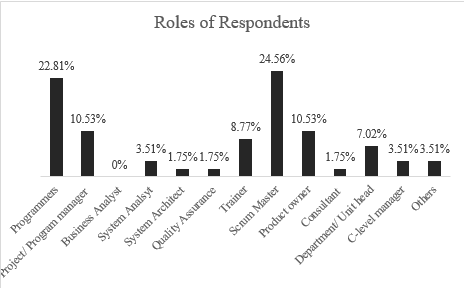
\includegraphics[]{Roles of the respondents.png}
\caption{Roles of the Respondents.\label{roles}}
\end{figure}

\subsection{Work Experience of the Respondents}
The work experience of each respondent with the agile development is asked to report in the survey. As this is one of the key factors to examine the quality of the responses. Moreover, this research is focused on the agile practices and agile development so experience with the agile development is essential hence the respondents were asked to indicate their work experience with agile development methodologies. The analysis of the work experience of the respondents showed that 33.33\% of the respondents are well experienced with 6-10 years of agile development. 22.8\% of the respondents have 1-3 years of experience. About 17.54\% of the respondents are experienced between 3-6 years with the agile development. 15.79\% of the respondents are professionals with the experience of agile development for more than 10 years. Whereas only 10.53\% of the respondent’s population have experienced less than 1 year. This implies that almost two-thirds of the participant (66.66\%) have experience for more than 3 years with the agile software development. Hence, based on work experience of the respondents the overall response to this questionnaire was satisfactory. For a clear overview, the work experience of the respondents is presented in figure \ref{work experience}.
\begin{figure}[h]
\centering
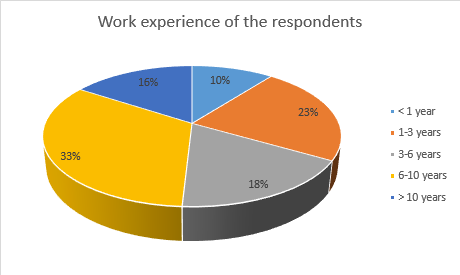
\includegraphics[]{Work experience.png}
\caption{Work Experience of the Respondents. \label{work experience}}
\end{figure}

\subsection{Industry domain of the respondents}
Respondents were asked to provide their industry domain in the questionnaire. Figure \ref{domain} represents the industry domains of the responses about 33.33\% of the respondents are from independents software vendors. The second largest group is telecom with 22.81\%. The third largest group of the respondents are from research and development with 10.53\%. Both the media entertainment and financial services contributed 8.77\% individually. These were followed by the health care 7.02\%, government 3.51\%, military 1.75\% and other 3.51\%. For this particular research, it is mainly focused on the agile development process and most of the data is collected from the industry domains related to independent software vendors, telecommunication, and research and development so this analysis provides that most of the collected data are reliable for this research.
\begin{figure}[h]
\centering
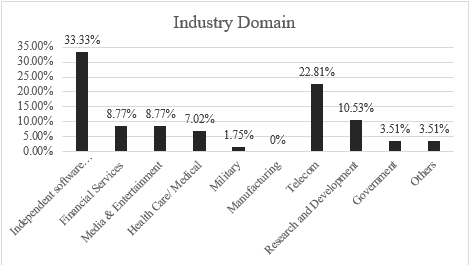
\includegraphics{Domain of industries.png}
\caption{Domain of Industries. \label{domain}}
\end{figure}
\subsection{Distribution of the team members}
Respondents were asked to report their experience with the distribution of their team members. The below presented figure \ref{distribution} represents the responses of the respondents regarding their team distribution.
\begin{figure}[h]
\centering
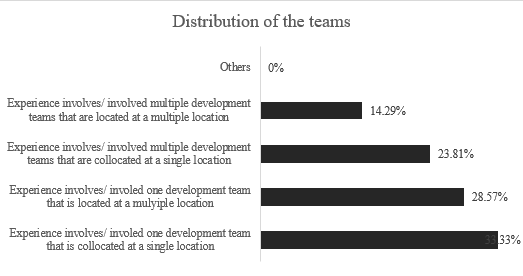
\includegraphics[height=5cm]{distributed teams.png}
\caption{Distributed teams. \label{distribution}}
\end{figure}


\subsection{Development types of the industry}
Respondents were asked to report the development type of the industry. The type of development during their experience. Market driven for the large open market has received 35.71\% of all the responses being the highest. A detail description of all the development types of the industries of the respondents is represented in figure \ref{development type}.
\begin{figure}[h]
\centering
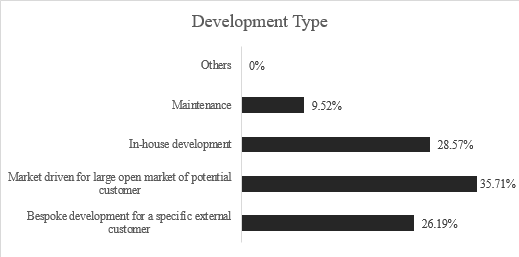
\includegraphics[height=7cm]{Development type.png}
\caption{Development type of the industry responded by the respondents. \label{development type}}
\end{figure}

\subsection{Usage of Agile Practices in the Industry}
The responses of the respondents were analyzed to determine the frequency of the use of agile practices. Based on the collected data the response rate of use of each individual practice is calculated and presented in figure \ref{usage}.
\begin{figure}[h]
\centering
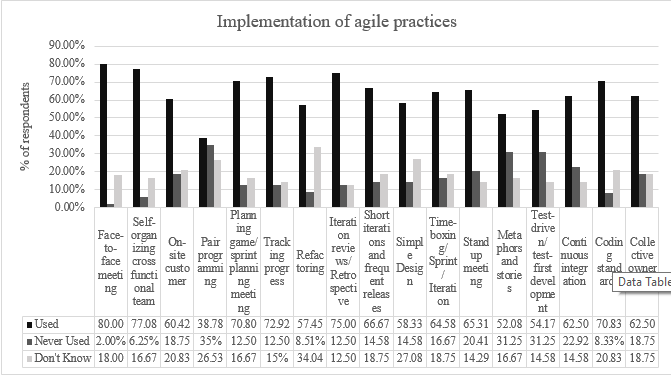
\includegraphics[width= 14cm]{usage.png}
\caption{Implementation of Agile practices mentioned by the respondents. \label{usage}}
\end{figure}

\newpage
The mean ranks of the practices were calculated using statistical analysis method called Friedman test as mentioned in section 3.5. C. Robson \cite{robson_real_2016} reports that Friedman test is related simple to compute manually but with computer assistance seems little reason to prefer it when the data in a form. Focusing on the perfections of the research authors preferred the use of statistical analysis with using SPSS (software 9version 23). The access to this software is provided by the university moreover, the reason for choosing this tool is that it has many books available for self-learning and this tool also suggested by C. Robson for statistical analysis \cite{robson_real_2016}. The following table \ref{mean ranks} represents the mean ranks of each practice calculated using Friedman test.
\begin{longtable}{|p{5cm}|p{4cm}|}
\caption{Mean Ranks after performing Friedman Test.  \label{mean ranks}}\\ \hline
\textbf{Agile practice} & \textbf{Mean Rank}\\ \hline
1. Face-to-face meeting&	7.68\\ \hline
2. Self-organizing cross functional team &	8.04\\ \hline
3. On-site customer&	9.21\\ \hline
4. Pair programming&	11.30\\ \hline
5. Planning game/ sprint planning meeting&	8.40\\ \hline
6. Tracking progress&	8.19\\ \hline
7. Refactoring&	10.07\\ \hline
8. Iteration reviews/ Retrospective&	7.95\\ \hline
9. Short iterations and frequent releases&	8.87\\ \hline
10. Simple Design&	9.59\\ \hline
11. Time-boxing/ Sprint/ Iteration&	9.13\\ \hline
12. Stand up meeting&	8.78\\ \hline
13. Metaphors and stories&	9.89\\ \hline
14. Test-driven/ test-first development&	9.61\\ \hline
15. Continuous integration& 	8.84\\ \hline 
16. Coding standards&	8.37\\ \hline
17. Collective ownership&	9.07\\ \hline
\end{longtable}
To align the agile practices in a particular order neither the results of the mean ranks nor the frequency of the most used agile practices is not sufficient because the mean ranks are calculated based on the frequency, mean and variance. So these mean ranks can only be subjected to know the most used practices in the industry through ranking.

Thereby, to retrieve the order of the agile practices authors performed a deeper analysis on the data extracted from the provided timeline in the questionnaire. There each informer aligns the agile practices in a distinct order in the timeline. Hence, there is no significant relationship between the responses of the respondents and so extreme care is taken while performing the analysis of this data related to the timeline. Both the authors are involved cautiously during this critical analysis. The analysis was performed through inspecting each individual agile practice. Based on the extracted data from the timeline each agile practice is investigated with the pre implemented and post implement agile practices. With this, the authors could figure out the practices that are implemented before a particular practice and also the practices that are implemented after a particular practice. With this particular data, each agile practice is examined to figure out its pre implemented and post implemented agile practices from all the respondents in order to align the practices in a certain order. The analysis and results of each agile practices are tabulated in table \ref{analysis of practices}. Here in the table \ref{analysis of practices} if observed it shows that of the respondents have indicated the use of self-organizing teams after P1(face to face meeting). Similarly, 4.64\% of the respondents had indicated self-organizing teams after P3(on-site customer) which further indicates that only 4.64\% of respondents used on-site customer after self-organizing teams and so on. Hence based on this analysis and response rate of the respondents extracted from the timeline these 17 agile practices are aligned in a particular order.
\begin{sidewaystable}
\tiny
\centering
\caption{Analysis of practices. \label{analysis of practices}}
\label{practices}
\begin{tabular}{|l|p{2cm}|l|l|l|l|l|l|l|l|l|l|l|l|l|l|l|l|l|l|}
\hline

 & \begin{tabular}[c]{@{}l@{}}Agile\\   Practices\end{tabular} & \begin{tabular}[c]{@{}l@{}}Total\\   Used (\%)\end{tabular} & P1 & P2 & P3 & P4 & P5 & P6 & P7 & P8 & P9 & P10 & P11 & P12 & P13 & P14 & P15 & P16 & P17 \\ \hline
1 & \begin{tabular}[c]{@{}l@{}}Face\\   to Face\\ communication\end{tabular} & 80 & - & 0 & 0 & 0 & 0 & 0 & 0 & 0 & 0 & 0 & 0 & 0 & 0 & 0 & 0 & 0 & 0 \\ \hline
2 & \begin{tabular}[c]{@{}l@{}}Self-organizing\\   teams\end{tabular} & 77.08 & \begin{tabular}[c]{@{}l@{}} \textbf{88.03}\end{tabular} & - & 4.64 & 0 & 0 & 3.8 & 0 & 1.2 & 0 & 0 & 0 & 0 & 0 & 0 & 0 & 0 & 2.33 \\ \hline
3 & \begin{tabular}[c]{@{}l@{}}On-site\\   customer\end{tabular} & 60.42 & 4.62 & \begin{tabular}[c]{@{}l@{}} \textbf{83.18}\end{tabular} & - & 0 & 4 & 0 & 0 & 8.2 & 0 & 0 & 0 & 0 & 0 & 0 & 0 & 0 & 0 \\ \hline
4 & \begin{tabular}[c]{@{}l@{}}Time\\   boxing\end{tabular} & 64.58 & 0 & 0 & \begin{tabular}[c]{@{}l@{}}\textbf{53.22}\end{tabular} & 0 & 12.68 & 0 & 0 & 0 & 0 & 0 & - & 13.88 & 6.12 & 0 & 7.5 & 0 & 6.62 \\ \hline
5 & \begin{tabular}[c]{@{}l@{}}Planning\\   game\end{tabular} & 70.83 & 0 & 0 & 0 & 0 & - & 0 & 0 & 0 & 11.21 & 0 & \begin{tabular}[c]{@{}l@{}}\textbf{74.03}\end{tabular} & 0 & 0 & 0 & 8.23 & 5.32 & 1.21 \\ \hline
6 & \begin{tabular}[c]{@{}l@{}}Simple\\   Design\end{tabular} & 58.33 & 0 & 0 & 0 & 0 & \begin{tabular}[c]{@{}l@{}}\textbf{100}\end{tabular} & 0 & 0 & 0 & 0 & - & 0 & 0 & 0 & 0 & 0 & 0 & 0 \\ \hline
7 & \begin{tabular}[c]{@{}l@{}}Tracking\\   progress\end{tabular} & 72.92 & 0 & 0 & 0 & 0 & 0 & - & 0 & 3.42 & 3.07 & \begin{tabular}[c]{@{}l@{}} \textbf{68.16}\end{tabular} & 0 & 4.33 & 0 & 0 & 6.33 & 0 & 14.69 \\ \hline
8 & \begin{tabular}[c]{@{}l@{}}Coding\\   standards\end{tabular} & 70.83 & 6.23 & 9.23 & 7.69 & 13.68 & 0 & \begin{tabular}[c]{@{}l@{}}\textbf{60}\end{tabular} & 0 & 0 & 0 & 0 & 0 & 0 & 0 & 3.17 & - & 0 & 0 \\ \hline
9 & \begin{tabular}[c]{@{}l@{}}Iteration\\   review\end{tabular} & 75 & 0 & 0 & 2.54 & 0 & 2.6 & 0 & 0 & - & 1.9 & 0 & 0 & 0 & 0 & 2.96 & \begin{tabular}[c]{@{}l@{}} \textbf{90}\end{tabular} & 0 & 0 \\ \hline
10 & \begin{tabular}[c]{@{}l@{}}Daily\\   standups\end{tabular} & 65.31 & 9.7 & 5.49 & 4.7 & 0 & 0 & 4.88 & 0 & \begin{tabular}[c]{@{}l@{}}\textbf{74}\end{tabular} & 1.23 & 0 & 0 & 0 & 0 & 0 & 0 & 0 & - \\ \hline
11 & \begin{tabular}[c]{@{}l@{}}Continuous\\   integration\end{tabular} & 62.5 & 0 & 0 & 0 & 13.48 & 0 & 0 & 0 & 7.66 & 0 & 0 & 0 & 0 & 0 & - & 5.9 & 2.36 & \begin{tabular}[c]{@{}l@{}}\textbf{70.6}\end{tabular} \\ \hline
12 & \begin{tabular}[c]{@{}l@{}}Frequent\\   releases\end{tabular} & 66.67 & 0 & 0 & 4.23 & 0 & 2.69 & 0 & 0 & 4.79 & - & 0 & 0 & 0 & 0 & \begin{tabular}[c]{@{}l@{}}\textbf{ 85}\end{tabular} & 2.12 & 0 & 1.17 \\ \hline
13 & Metaphors & 52 & 0 & 0 & 5.4 & 0 & 6.7 & 0 & 0 & 0 & \begin{tabular}[c]{@{}l@{}}\textbf{83}\end{tabular} & 0 & 2.6 & - & 0 & 0 & 0 & 0 & 2.3 \\ \hline
14 & \begin{tabular}[c]{@{}l@{}}Collective\\   ownership\end{tabular} & 62.5 & 5.9 & 6.3 & 0 & 0 & 0 & 0 & 0 & 5.17 & 0 & 0 & 0 & \begin{tabular}[c]{@{}l@{}}\textbf{82.63}\end{tabular} & 0 & 0 & 0 & - & 0 \\ \hline
15 & Refactoring & 57.45 & 0 & 0 & 0 & 0 & 7.8 & 0 & - & 0 & 0 & 0 & 0 & 0 & 0 & 13.6 & 15.6 & \begin{tabular}[c]{@{}l@{}}\textbf{63}\end{tabular} & 0 \\ \hline
16 & TDD & 45.83 & 13.5 & 9.23 & 15 & 12.7 & 17 & 0 & 0 & 0 & 0 & 11 & 0 & 0 & - & 8.9 & 7 & 0 & 6 \\ \hline
17 & \begin{tabular}[c]{@{}l@{}}Pair\\   programming\end{tabular} & 38.78 & 11 & 8.9 & 0 & - & 13.5 & 0 & 9.78 & 0 & 0 & 8.2 & 9.23 & 0 & 15 & 0 & 17 & 0 & 7.39 \\ \hline
\end{tabular}
\end{sidewaystable}
\newpage
While aligning the practices in the order, the practices like TDD and pair programming are not widely implemented in the industry as per the collected data. These practices had also shown variances in the order of implementation. So for aligning this kind of practices authors considered the experience, roles of the respondents and mean ranks. Experience with more than six years and the respondents experienced with more than two roles were given much importance than the responses with experience less than one year. Some of the respondents who used pair programming did not use TDD. So to prioritize these kind of practices mean ranks are used. Keeping these cases in view mean ranks are calculated to understand the importance of agile practice while prioritizing the practices.  The reason for using mean ranks is that the most used agile practices will help in improving the agility of the software development process hence mean ranks also played a role in aligning the agile practices in a certain order. But the preliminary data used for every agile practice to aligning them in a particular order is strictly based on the data extracted from the timeline (refer Appendix \ref{appendix B}) which is reported by the respondents. 

Based on the results achieved the agile practices are aligned in a specific order with the description of results and reasons of placing that practice at that particular place within the 17 agile practices.
\begin{enumerate}
\item \textbf{Face-to-face meeting:} 80\% of the respondents reported the use of face-to-face communication and also all of them indicated that the first implemented agile practice is face-to-face communication in their respective timeline. Hence, this practice is first prioritized over the 17 agile practices.
\item \textbf{Self-organizing cross functional teams:} 77.08\% members of the respondents had reported the use of self-organizing teams in which 88.03\% of respondents reported this practice after face-to-face communication. Moreover, out of 11 respondents who implemented this practice having experience between 6-10 years, 10 of them reported this practice after face-to-face communication. One of the programmers with experience between 6-10 years indicated that this practice is widely used from more than six years with a small variation of team size between 6-8 members over the past years.
\item \textbf{On-site customer:} Surprisingly 39.58\% respondents did not indicate the use of this particular agile practice but out of remaining 60.42\% of the respondents 83.18\% of them reported on-site customer after the self-organizing teams in their respective timelines and one of the c-level manager commented that in an agile development on-site customer is essential in the development process so that the customer can be consulted at any time for any changes in the requirements or process.
\item \textbf{Time boxing/ Sprint/ Iteration:} 64.58\% of respondents had indicated the used of time boxing in which 33 (53.22\%) of them indicated that time boxing is implemented after the on-site customer. Moreover, two of the respondents having more than 10 years’ of experience had mentioned that fixing time period for each activity is essential to meet the deadlines and also one of the respondent programmer having more than 6 years of experience described that the development process would be more effective if time boxing is implemented individually to frame personal tasks within a smaller time frame to stay on schedule.
\item  \textbf{Planning game/ Sprint planning meeting:} 70.83\% of the respondents reported the use of sprint planning in which 74.03\% of the respondents reported the use of sprint planning after the time boxing so that each activity is planned with respect to the time frame for that particular activity to develop the required essential features for developing the project.
\item \textbf{Simple Design:} This particular practice showed interesting results that only 58.33\% of the respondents implemented this practice in the organization where as 27.08\% reported they are not aware of this particular practice. But surprisingly all of the 58.33\% of respondents have indicated the use of this practice after the sprint planning activities. Eight of the respondents including the scrum masters and project managers had commented similarly that implementation of this practice is essential to figure out simplest solutions in order to save time.
\item \textbf{Tracking progress:} Tracking progress is one of the essential practice in any agile software development process. Out of 72.92\% respondents, 68.16\% of respondents indicated the use of this practice in the timeline next to simple design. One of the respondents having 6-10 years of experience described that their organization use JIRA boards and reported that these boards are not effective. He also suggested that additional use of burndown charts is important to track the actual development progress.
\item \textbf{Coding Standards:} About 70\% of the respondents have indicated the use of this practice in which 58.6\% of the respondents are well experienced with more than 6 years of experience. For this particular practice, more than 60\% of them reported the practice after the tracking progress in their respective timelines.
\item \textbf{Iteration Reviews/ Retrospectives:} 90\% of the respondents who indicated the use of this particular practice has reported this practice in the timeline after the coding standards. One of the trainer among the respondent’s experience for more than 6 years of agile development mentioned that iteration reviews are performed after each iteration to review the developed project to discuss threats to process efficiency and also mentioned that iteration reviews help to identify the gaps in the development process. Also, a project manager commented that “Iteration reviews should be done before any release of the developed software to find any hidden flaws”.
\item \textbf{Daily Stand-up meetings:} Standup is one of the essential features in scrum development methodology. The response rate for this practice is 65.31\% which indicated that approximately 35\% of the respondents did not use this particular practice. Being one of an essential practice in agile this practices is not yet being put into practice completely as per the collected data. One of the potential reasons is that not all of the respondents are following scrum methodology. Over 74\% of those who indicated the use of this practice reported it after the iteration reviews and interestingly eight of the respondents had commented on this practice. All of the respondents reported similar comments like “mandatory”, “always used in some form” etc. The respondents who had commented on this practice have different years of experiences under their belt. Three of them have 6-10 years, one more than 10 years, two of them with 3-6 years and other two of them have 1-3 year of experience. One of the comment “very important” is posted by a project manager from an international company.
\item \textbf{Continuous Integration:} Of the 62.5\% participants who responded to this practices more than 70\% of people had marked this particular practice after the standups. One of the programmers having experience for more than 10 years mentions in the comment that “Even continuous deployment is also in use”. A continuous deployment is an approach where the software is developed in short cycles so that every change that passes the automated test is deployed automatically to the production line for better performance in the developed code.
\item \textbf{Frequent Releases/ Short Iterations:} In total 66.67\% of the respondents have implemented this practice in their development process and a slightly more than 85\% of the respondents had marked this practice after the continuous integration. One of the project managers commented that in their organization they “use short iteration but not the frequent releases”.
\item \textbf{Metaphors \& Stories:} Interestingly 48\% of the informants did not indicate the use of metaphors, 52\% of the informants only indicated the use out of which 83\% of respondents had marked this practice continuous integration. None of them has given any comment regarding this particular agile practice.
\item \textbf{Collective Ownership:} More than half of the respondents (62.5\%) had reported the use of this particular practice but most of the respondents had reported this practice at the end of the timeline before refactoring and after metaphors and stories. 18.75\% of the respondents did not use this practice and another surprising factor with particular practice is that the same equal number of respondents (18.75\%) are not aware of this practice.
\item \textbf{Refactoring:} Interestingly 34.04\% of the respondents are not aware of this particular practice but 57.45\% have used this and reported it at the end of time line but 5 of the respondents had marked use of this practice after simple design. Among five, three of the respondents are having less than three years of experience.
\item \textbf{Test Driven Development (TDD):} 45.83\% of the respondents had never used this practice in which 14.58\% of them are unaware of this practice. The respondents who had marked the use of this practice did not show any cumulative relation to other practices. Each respondent had marked the use of this practice at the different time. The same situation is faced with the least used practice i.e. pair programming. Hence to align these both practices it had been challenging, so mean ranks are compared to check for the most used practice among TDD and pair programming. TDD was more used than pair programming this implies the use of TDD contributes better agility in the development process than pair programming. Therefore, authors decided to align TTD before pair programming for an effective development process.
\item \textbf{Pair Programming:} Pair programming, this is the least used practice among the 17 agile practices by the respondents. Only 38.78\% of the respondents indicated that they had used this practice and almost the same number of respondents (34.69\%) mentioned that they never used this practice before. 26.53\% of the respondents indicated that they are unaware of this practice. Two of the respondents reported that “Pair programming is a good practice but never used it” and another response was “used very sparingly throughout the process”.
\end{enumerate}

The above mentioned 17 agile practices are aligned in a particular order for an efficient and effective software development process and also to attain the benefits of agile development. These 17 agile practices are aligned after performing a deep analysis and synthesis of collected data through conducting the survey. “With the growth of agile adoption, the question of why to adopt agile practice was quickly being replaced with how to adopt agile practices” \cite{sidky_structured_2007}. This particular research can provide potential answers on how to adopt agile practices in an efficient way. The above mentioned order of agile practices can benefit the organizations in many several ways. The benefits of implementing the agile practices in this particular order will be discussed in the further sections. Aiming for a more precise research and to contribute the best knowledge to this particular field of study, authors had decided to continue their research at an advanced level to validate their proposed order of agile practices through conducting interviews with the expert professionals in agile development.
\subsection{Results from open-ended questions}
The first open ended question provided in the questionnaire to the respondents was regarding the measure of success with their experience in the agile development process. This particular question was intended to gather the benefits and success of implementing agile practices in their organization. Most of the respondents responded the measure of success in a positive manner. 80.44\% of the respondents reported that their experience with the implementation of the agile practices was successful (refer figure 11). A variety of perspectives on the measure of success were expressed by the respondents few of them were:

\textit{“Measure of success=5(1-5) with good team collaboration quality product can be delivered. Collective ownership contributed to project success”.}

\textit{“Better quality and happier staff with increased productivity, reduced defects thereby reducing time spent on defects. Agility was my main attraction to the methodology”.}

\textit{“Delivering working software more quickly with the happier team which reduces the stress/ pressure on the team. Fewer defects to fix with reduced emphasis on deadlines so the team enjoys build software that clients love. On a scale of 1 to 10, I can give 8/10”.}

\textit{“Value delivered; stakeholder satisfaction; the great rate of learning with minimal product issues; financial success with on-time delivery; a measure of success maximum extent”.}

Similarly, most of the respondents have reported their measure of success with respect to their agile development process. All the responses of the respondents were analyzed and the benefits regarding the use of agile practices are reported below:
\begin{itemize}
\item Increased team collaboration and ownership.
\item	Enhanced coordination and communication between the team members.
\item	Frequent releases of the developed product after each iteration.
\item	Decrease in production issues.
\item	Able to adopt changes frequently with on-time delivery.
\item	Happy customers and happy teams.
\item	Transparency in the development process for all the stakeholders.
\item	Focus on both the customer and business value.
\item	Improved quality with reduce in cost.
\item	Flexibility and adaptability in the development process.
\item	Implementation of code refactoring.
\item 	Knowledge sharing with the implementation of daily status meetings.
\item	Early access to test the software.
\item	Minimal documentation.
\item	Reduce in defect density.
\item	Constant feedback on products and process for better enhancements.
\item	Better risk management.
\item	Better control over the development process and project.
\item	Increased team morale.
\item Velocity measurement and control charts help team to develop.

\end{itemize}

Correspondingly, the respondents were asked to report the limitation/ challenges faced while adopting the agile practices. This question was intended to gather the limitations/ challenges faced while adopting the agile practices in their software organization. From all over the responses the most common challenges faced by the practitioners are identified through performing a detail investigation on the responses and these challenges faced by the practitioners. A variety of perspectives on limitations/ challenges were expressed by the respondents some of them are described below:

\textit{“Agile methods shift focus towards a true collaborative "team" as opposed to a group of individuals working on independently on parts of the same project. This creates a need for a broader "soft skills" set around key areas such as communication and teamwork. Some software development companies have invested heavily as a part of their team's professional development. Pure technical skill is not the *only* measure for a high performing agile team member, and these skills takes time to develop”.}

\textit{“Getting the agile mindset into the organization is a bigger challenge. Sometimes documentation is needed when you are working on support project whereas in agile documentation scope is limited. Team members who are not familiar with the agile practices take longer learning time”.}

\textit{“Most of the time is spent on "agile administration", such as debating on whether to have an electronic board or not. Describing stories / tasks often fail, because the short descriptions are misunderstood by team members. Continuously improving the agile process is complex, especially if there is no dedicated scrum master in the team. The official scrum master is also a developer and spends most time developing the code. Occupying testers / business users within the team at the initial stages of the sprint (scrum) is often harder”.}

\textit{“Not all agile practices can be adopted. A lot depends on the type of project you are working on and the phase of the project you are in. We don't refactor that often because the priority was on developing new features, not existing ones. The culture of the organization plays a major role in Agile adoption. We can't go for Agile practices when users want to do production parallel testing for the whole project”.}

Similarly, most of the respondents have reported their challenges with respect to their agile development process. All the responses of the respondents were analyzed and the limitations/ challenges regarding the use of agile practices are reported below:
\begin{itemize}
\item Depending on project domain, project type and phase of the project, agile practices should be adopted. Not all agile practices can be implemented at once. This requires a superior decision maker.
\item 	Extra effort is needed to maintain good interaction between the customer and development team to develop the product as per customer needs.
\item	Due to minimal documentation, the scope is limited and sometimes documentation is needed when working on support project.
\item	Additional heavy investment and extra effort is needed to train the agile team and also the training takes longer time.
\item	A broader sort skills are needed for effective communication and team work.
\item	Adopting agile mindset and maintaining agile culture is challenging in an outsourced environment.
\item	Dealing with legacy code possess additional challenges to teams.
\item	Parallel testing is not flexible with agile practices.
\item	More elitism caused more trouble.
\item	Developing and structuring user stories is challenging sometimes. Describing stories often fail because short descriptions are misunderstood by team members.
\item	Without dedicated agile administration continuously improving the agile process is a bigger challenge and threat to the entire team.
\item	Changes come hard and people are skeptical sometimes.
\item	Frequent build sometimes leads to code breakage.
\item	Communication challenges between globally distributed teams.
\end{itemize}

In the next open ended question, the respondents were asked to report their reasons for adopting the practices in that particular way/ order with respect to their reported order of practices. This question was intended to gather the reasons behind adopting the agile practices in that particular way or order. From all over the responses the most common reasons for implementing agile practices by the practitioners are identified through performing a detail evaluation on the responses reported by the respondents. A variety of perspectives on implementing agile practices in a particular way/ order were expressed by the respondents are described as follows:

\textit{“Agile practices need to be aligned in a particular order for successful implementation of agile practices and to eliminate integration issues”.}

\textit{“They need to be aligned in particular order to complete all the assigned user stories in stipulated time”.}

\textit{“To increase efficiency by having more control over planning process and also to eliminate unnecessary actions. Thereby to save time, budget and to improve the quality”.}

 Most of the respondents have reported their reasons with respect to their agile development process. All the responses of the respondents were studied and the reasons regarding the implementation of agile practices in a particular way/ order are reported below:
 \begin{itemize}
\item To increase efficiency and have more control over planning process by eliminating unnecessary actions.
\item	Agile administration containing executive supervisors decides the order of the agile practices which needs to be implemented.
\item	Alignment of agile practices is important to minimize the integration issues.
\item	Implementing of agile practice in a certain order help in faster execution, faster feedback and time to market.
\item	To shorten lead times and avoid delivering functionality which is no longer relevant.
\item	To save time, budget and improve quality in the development process.
\end{itemize}

The fourth question was asked to report whether any practices were terminated during the development process. This question was intended to gather reasons behind if any of the practices were terminated during the development process. All of the respondents except one reported similar statements that none of the practices were terminated during the development process. One responded who reported the termination of the practice reported that pair programming was terminated in their organization in the middle of the development process as this practice was not efficient moreover creating overheads with in the team.  Two of the respondents in spite of non-termination of practices comment in provided text field:
\begin{itemize}
\item One of the respondent reported that \textit{“In his experience most team members (especially developer) are often positive using agile practices and told that no practices were terminated”.}
\item Other respondent reported that \textit{“I don’t see any practices which were using in our project have been terminated. But on my personal account, I would terminate a practice if I find it redundant, doesn’t resolve any issue or uncertainties in the project”.}
\end{itemize}

The last open ended question was provided optionally to add additional remarks or comments regarding their adoption of agile practices with respect to their agile experience. Few of the respondents responded to this field thereby all the additional comments were gathered, analyzed and reported below. One of the impressive comment was 

\textit{“If you are aiming at a strategic adoption of ‘agile’ methods, it’s worth considering what Peter Drucker said: ‘culture eats strategy for breakfast’. Adoption of the process will not produce an agile culture; however, they will reinforce it. This is emphasized in the ‘agile manifesto’ where it states that ‘Individual and iterations’ need to VALUED MORE than ‘processes and tools’; the latter is important, but the former is more important. If you are implementing a cultural change, you need to be able to understand how to analyze the current organization culture. The motion of the ‘Cultural Web’ as a tool for analysis is useful here. Common wisdom is that this will take about three years and will cost 20-30\% of your team who will not be able to adjust. That matches our experience”.}

Additional comments provided by the respondents are
\begin{itemize}
\item	Agile needs to be modified or combined with other practices to fit the business needs.
\item Extreme care should be taken in the sprint planning meetings regarding the prioritization of user stories with a clear description of the requirements for each user story included in the product backlog. 
\end{itemize}

\section{Summary of the results}
In order to identify and understand the order of agile practices of agile maturity model implemented in the industry, a survey was conducted with the current software practitioners. Also, the benefits and limitations of implementing these agile practices in a certain order are known with this survey. After conducting the survey, the collected data is analyzed by using statistical and comparative analysis methods to attain reliable results. Analysis of the demographic results showed that 67\% of the respondents were having experience for more than three years. If observed clearly, 33\% of the respondents have experience of the respondents for more than 10 years in the field of agile software development. Therefore, with respect to the experience of the respondents, the summary of the results showed a positive sign indicating that the respondents have high enough experience to answer the questionnaire which means the collected answers from the respondents are reliable to perform the research. Moreover, the respondents are located from different geographical locations adding an advantage of analyzing the data from different continents thereby understanding the agile development process followed by the organization from all over the world. Each of the respondents possesses different roles are from different levels this helped in understanding the perspectives of each respondent with respect to their designation. If observed in the previous section (4.2.2) the rate of responses of the respondents from different roles within the organizations are analyzed and reported. The responses were gathered from different industry domains in which the highest response rate was from independent software vendors, this helped in identifying and understanding of the implementation of agile practices from medium and large scale software industries.

54.35\% of the respondents felt that the adoption of agile practices was successful moreover 26.09\% of the respondents reported that according to them the adoption of the agile practices was very successful. In the bellow pie chart \ref{success rate}, a detail perception of all the respondents regarding the success of adoption of agile practice is described in detail.
\begin{figure}[h]
\centering
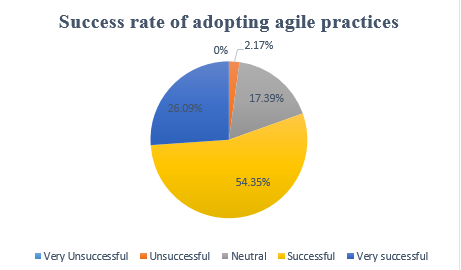
\includegraphics[]{success rate.png}
\caption{Success rate of adopting agile practices. \label{success rate}}
\end{figure}

In depth analysis on the 17 agile practices used for this particular research resulted that face to face communication and iteration reviews are the most frequently used practices in the industries followed by self-organizing teams, tracking progress, coding standards, planning game, standup, continuous integration, frequent releases, collective ownership, time boxing, onsite customer and simple design. Practices like TDD, metaphors, refactoring and pair programming are the least used practice among the 17 agile practices according to the collected responses. After carefully reviewing the agile practices reported by the respondents the agile practices are aligned in a particular order so that implementation of these agile practices in this particular order can enhance that software development process attaining the actual benefits of agile development. These 17 agile practices are aligned after performing a deep analysis and synthesis of the collected data in the following order.
\begin{table}[h]
\centering
\caption{Derived order of agile practices}
\label{order}
\begin{tabular}{|l|l|}
\hline
\textbf{ID} & \textbf{Agile Practices}               \\ \hline
1.          & Face-to-face meetings                  \\ \hline
2.          & Self-organizing Cross Functional Teams \\ \hline
3.          & On-site Customer                       \\ \hline
4.          & Time Boxing                            \\ \hline
5.          & Planning game/ Sprint Planning Meeting \\ \hline
6.          & Simple Design                          \\ \hline
7.          & Tracking Progress                      \\ \hline
8.          & Coding Standards                       \\ \hline
9.          & Iteration Reviews                      \\ \hline
10.         & Standup Meetings                       \\ \hline
11.         & Continuous Integration                 \\ \hline
12.         & Frequent Releases                      \\ \hline
13.         & Metaphors \& Stories                   \\ \hline
14.         & Collective Ownership                   \\ \hline
15.         & Refactoring                            \\ \hline
16.         & TDD                                    \\ \hline
17.         & Pair Programming                       \\ \hline
\end{tabular}
\end{table}

In the next part of the questionnaire, it consists of five open ended question to gather the practitioner’s perspective on the benefits and limitations of implementing the agile practices in the software development process. The first part of the open ended question aims at knowing the benefits and measure of the success of implementing agile practices. The results of the analysis showed that 80.44\% of the respondents felt that implementation of agile practice was successful. Most of the responded that the agile is flexible and adaptable to change in requirements. The essential benefits of the agile development are frequent releases of the shippable product. Several other identified benefits of implementing agile practices are documented in the previous section (4.2.8).
Next part of the open ended question focus on understanding the challenges faced by the software practitioners due to the adoption of agile practices and also the respondents were investigated if any of the adopted agile practices are terminated during the development process due to some particular reasons. The respondents were asked to report the difficulties faced during the process if agile development. Several challenges were identified after performing the analysis. The results are documented in the section 4.2.8 out of which most commonly faced challenges by the practitioners due to agile development are regarding selecting and adopting of agile practices in a particular order based on their development type of project, issues with the training of the agile to the practitioners who are new to agile development, time constraints, and issues with the agile administration. In detail, all the challenges reported by the respondents were reported in the previous section (4.2.8). None of the respondents reported the termination of the agile practices during the agile development except one. With this, the objective of conducting the survey is completely achieved. 


\section{Results from Interviews}
\subsection{Interviewee background information}
Three interviews have been conducted for validating the proposed order of practices. The background information of all the interviewees with their experience of agile development is described in this section.
\subsubsection{Introduction of interviewee 1}
The first interviewee has experience of 22 years in the IT industry. He has taken several roles and responsibilities in the field of software engineering in past years. He has 13 years of experience in the field of Agile software development and presently pursuing a role of Agile coach. He reported that he is responsible for setting the ground rules and regulations for developing the project. The duration of interviewing him took about 33 minutes.
\subsubsection{Introduction of Interviewee 2}
This particular interviewee started his career as a front-end web developer and presently working as a project manager since 2006. This interviewee is a PMI agile certified practitioner. Presently he is leading a software vendor project started in 2014. The interview lasted for 24 minutes.
\subsubsection{Introduction of Interviewee 3}
Interviewee3 has experience with the agile software development for more than 7 years and started her career in the year of 2005. She is a program manager in an international IT company. The interview with her took about 20 minutes.
\subsection{Results and analysis of Interviews}

From the background information mentioned in the section, it is clear that all the three practitioners are well experienced with in the field of agile software development. All of the interviews are conducted through video calling as per their convenience. With their prior permissions, the interviews were recorded with the means of audio tapes. Later these audio tapes carefully listen and are transcribed into a text format. As mentioned earlier in the research methodology the interviews were conducted in a semi-structured format so that a clear explanation of the required information can be gathered.

All of the three respondents said that they did not find any difficulties in understanding the phrases and terminology used in the checklist and also told that they were familiar with all the mentioned agile practices. Among these three, the first (agile coach) and second (project manager) interviewees have stated that metaphor should be implemented before simple design so that the entire development team will be aware of the requirements specified by the customer. Moreover, they mentioned that a clear definition of the requirement is essential to building the product as per the customer needs so that rework can be avoided thereby saving time which is very important. Owing to this suggestion the agile practice ‘metaphor’ is rearranged and placed in between the sprint planning meeting and simple design. Thereby, with this rearrangement of practices the order of agile practices is validated and framed in a form of checklist. 

With respect to the fourth question in the questionnaire regarding the benefits and challenges, all the three interviewees expressed their distinct opinions regarding the proposed order of agile practices. This collected data is analyzed using thematic analysis method. This analysis is performed in a step by step process as recommended by Lacey et.al \cite{lacey_qualitative_2001}.

Initially transcription of the data is done through making notes from the audio tapes. Without missing any data, the transcription is done individually for all the three responses. Again the transcribed data is carefully examined for understanding the collected data and also to check if any data is missed. In the next process, the data collected from all the three respondents is integrated for the ease of analysis. Later the coding for the transcribed data is done. Several distinct codes were identified and each code is assigned to a different color for easy identification of the relevant codes. In the next process, the identified codes possessed variable frequencies, the most frequently identified codes are then categorized into themes. The following table \ref{codes} represents the identified codes and are then categorized into their respective themes.
\begin{table}[h]
\centering
\caption{Identified Codes and themes}
\label{codes}
\begin{tabular}{|l|l|}
\hline
\textbf{Codes Identified} & \textbf{Themes}                               \\ \hline
On time Delivery          & \multirow{5}{*}{Effectiveness of the process} \\ \cline{1-1}
Fixed Deadlines           &                                               \\ \cline{1-1}
Defined standards         &                                               \\ \cline{1-1}
Clear Requierements       &                                               \\ \cline{1-1}
Development Process       &                                               \\ \hline
Clear Understanding       & \multirow{3}{*}{Enhanced Communication}       \\ \cline{1-1}
Customer Involvement      &                                               \\ \cline{1-1}
Self-organizing           &                                               \\ \hline
Daily review meetings     & \multirow{3}{*}{Multiple Themes}              \\ \cline{1-1}
Period releases           &                                               \\ \cline{1-1}
Review meetings           &                                               \\ \hline
\end{tabular}
\end{table}

Based on the identified codes two themes have been generated in which they are categorized into the effectiveness of the process, enhanced communication, and multiple themes. Whereas multiple themes addresses both enhanced communication and effectiveness of the process. All the identified codes discuss the benefits of implementing the agile practices in the proposed order. None of the respondents have reported the challenges regarding the implementation of agile practices for this particular order.
\subsubsection{Analysis and results regarding the benefits}
Based on the analyzed data, 11 codes were identified and were categorized into three themes. In this section, the mapping of codes with its themes are generalized.

\textbf{Effectiveness of the process:} The clear requirements, fixed deadlines, defined standards, on time delivery and development process are mapped into this particular theme. Among three of the respondents, one had reported that “with clear requirements and fixed deadlines the agile development process can be improved and the product can be delivered on time”. Involvement of the customer in the initial stage itself is an essential practice as it helps in prioritizing the user stories in the product backlog. With this, the developers team can have a clear idea of the product which they need to develop and this also saves time and efforts of the developers avoiding unnecessary developments. Implementing time boxing helps in fixing the start and end date to the accomplish the project. Thereby delivering the project on time.

\textbf{Enhanced communication:} The codes clear understanding, customer involvement and self-organizing are mapped into this particular theme. One of the respondents reported that \textit{“According to me, frequent communication between the team members helps the team to be self-organized improving the collaboration of work between them. Customer involvement in the review meetings helps the team in assessing the developed product”}. Face-to-face communication will definitely improve the understanding between the team members as this is the best means of communication. Involvement of the customer in the sprint planning and review meetings helps the team in clearly understanding the specifications of the product. Moreover, it helps the developers to clarify any doubts or questions regarding the product specification due to the direct availability of the customer.


\chapter{Analysis and Discussion}
This section focuses on the observations and analysis of the collected data to answer the research question. Results that are achieved through conducting this survey will be mapped to its respective research question and research objective. Moreover, based on the achieved results an innovative checklist is framed and presented for the ease of software practitioners who are involved with the agile development methodologies.
\section{Answering the Research Questions}
\subsection{RQ1}
This research question is intended to identify the order of agile practices recommended in agile maturity models from the literature. To answer this question a literature review was conducted and the articles that describe various maturity models are extracted from the scientific databases. These several models were analyzed in detail and synthesized in order to identify the different agile maturity models with its set of agile practices. In total nine maturity models were extracted from the current literature. Each maturity model is carefully examined to retrieve its structure and set of agile practices. A comprehensive overview of each maturity model is presented in the results section 4.1. With an innovative approach this study has a unique characteristic of presenting the nine maturity models in a single table. According to authors knowledge, there are no similar studies presenting nine maturity models in a single study.

A very little was found in the literature regarding the analysis of agile maturity models. One study by Schweigert et.al \cite{schweigert_agile_2013} describes the currents status of agile maturity models and provide an approach to extract and analyze the agile maturity models. There are few studies which had compared utmost of five maturity models in their studies like Ozcan Top \cite{ozcan-top_assessment_2013} had made an attempt in assessing five agile maturity models. Whereas another study by Sidky \cite{sidky_structured_2007} had compared three agile maturity models and proposed a new maturity framework. But whereas this particular study is designed to extract and analyze nine maturity models identified in the literature. All the nine maturity models included in the study are compared and presented in section 4.1 which represents a logical structure of each maturity model with their set of agile practices. Thereby, adding an advantage of comparing the different agile maturity models with one another. After the analysis on nine maturity models one interesting finding was the practices like planning game, on-site customer and daily standups are suggested at the initial levels in most of the models. Another interesting finding is that in all nine maturity models there was no consistency found regarding the implementation of TDD and pair programming. But their ultimate aim of each maturity model is to guide the organizations in continuously improving their development process through a staged method. With this, the authors conclude that their first objective to identify the order of agile practices from the maturity models has been achieved successfully.
\subsection{RQ2}
The second research question aims at finding the order of agile practices that are implemented in the industries. To obtain this, a questionnaire was framed and the survey was conducted with the software practitioners who are experienced with agile development. Survey was performed in a structured professional manner under the supervisor guidance. The data is collected from the different practitioners located geographically from all over the world. The responses were collected from the targeted population each performing different roles and responsibilities. The collected data is analyzed by performing both the statistical analysis and comparative analysis. Friedman test was conducted to understand the most used using agile practices in the industries through mean ranks. Later on, in depth, critical analysis was performed to align the 17 agile practice in a particular order based on the collected data from the timeline, so as to attain the actual benefits of agile practices and presented in the following table \ref{derived}.
\begin{longtable}[h]{|l|l|}
\caption{Derived order of agile practices.\label{derived}}\\
\hline
\textbf{ID} & \textbf{Agile Practices}               \\ \hline
1.          & Face-to-face meetings                  \\ \hline
2.          & Self-organizing Cross Functional Teams \\ \hline
3.          & On-site Customer                       \\ \hline
4.          & Time Boxing                            \\ \hline
5.          & Planning game/ Sprint Planning Meeting \\ \hline
6.          & Simple Design                          \\ \hline
7.          & Tracking Progress                      \\ \hline
8.          & Coding Standards                       \\ \hline
9.          & Iteration Reviews                      \\ \hline
10.         & Standup Meetings                       \\ \hline
11.         & Continuous Integration                 \\ \hline
12.         & Frequent Releases                      \\ \hline
13.         & Metaphors \& Stories                   \\ \hline
14.         & Collective Ownership                   \\ \hline
15.         & Refactoring                            \\ \hline
16.         & TDD                                    \\ \hline
17.         & Pair Programming                       \\ \hline
\end{longtable}

Several studies conducted by Santos et.al \cite{santos_improving_2013}, R.Vijayasastry et.al \cite{vijayasarathy_agile_2008} and Begel et.al \cite{begel_usage_2007} had focused on usage of agile practices and their benefits. Whereas this particular study focuses on retrieving the implementation of agile practices in a certain order in the IT industries. The above mentioned order of agile practices was again validated through conducting interviews aiming for a more detail research and to contribute the best knowledge to this particular research area. With a view, that organizations can be beneficial with the actual benefits of implementing the agile practices in this particular way/ order. With this, the second objective is achieved also answering the RQ2.
\subsection{RQ3}
This respective question is intended to identify the benefits and limitations of implementing the agile practices. To answer this, respondents were provided with open ended questions to provide clear cut benefits and limitations which they have experienced during the implementation of agile practices. The collected qualitative data was analyzed for identifying the benefits and limitations. The most common benefit reported by the respondents was regarding the flexibility and adaptability of the agile development process with the acceptance of change in requirements even in the middle of the development process. Whereas one of the most common challenge reported was maintaining the agile culture throughout the development process. A detail results regarding the benefits and limitations are reported in the section 4.2.7. By this, the third objective O3 of the study is achieved.

The fourth objective O4 is to analyze the results obtained from the literature and survey to see if there are any commonalities and differences. The derived order of agile practices from the survey results are compared with the extracted agile maturity models to see if there exits any relevance or not. After careful examination of the order of agile practices obtained through a survey it showed some relevance with the Sidky Agile Measurement Index (SAMI). The maturity models are defined in different levels with a set of agile practices, if carefully observed the derived order from the survey results, the order of practices showed resemblance with the practices defined in SAMI with irrespective of their levels. Also when compared with Kent Beck’s study the results obtained from the survey had shown few commonalities. In his study if observed from the figure \ref{XP} the practices like on-site customer and planning game, collective ownership and refactoring, continuous integration and short iterations are linked together. Beck states that these combination of practices can improve the efficiency of the development process. This particular combinations of agile practices  was also found in the aligned order of agile practices from the results of survey.
\subsection{RQ4}
This question is framed to validate the proposed order of practices that are framed from the results of the questionnaire and the literature. This is validated through conducting interviews. Initially, an interview questionnaire is framed and this is cross verified with the supervisor for enhancements. Later with this questionnaire interviews are performed with well experienced agile software practitioners. The respondents accepted the proposed order which can be beneficial. But interestingly two of the Interviewees out of three suggested that metaphor needs to be rearranged between the sprint planning and simple design. As per the suggestions given by the respondents the proposed order of checklist is validated. The validated order of checklist is presented in table \ref{validated}. The validated order of practices will be helpful for the practitioners who are planning to adopt the agile practices, which would be beneficial to improve their productivity.
\begin{table}[h]
\centering
\caption{Validated order of practices}
\label{validated}
\begin{tabular}{|l|l|}
\hline
\textbf{ID} & \textbf{Agile Practices} \\ \hline
1. & Face-to-face meetings \\ \hline
2. & Self-organizing Cross Functional Teams \\ \hline
3. & On-site Customer \\ \hline
4. & Time Boxing \\ \hline
5. & Planning game/ Sprint Planning Meeting \\ \hline
6. & Simple Design \\ \hline
7. & Metaphor \& Stories\\ \hline
8. & Tracking Progress \\ \hline
9. & Coding Standards \\ \hline
10. & Iteration Reviews \\ \hline
11. & Standup Meetings \\ \hline
12. & Continuous Integration \\ \hline
13. & Frequent Releases \\ \hline
14. & Collective Ownership \\ \hline
15. & Refactoring \\ \hline
16. & TDD \\ \hline
17. & Pair Programming \\ \hline
\end{tabular}
\end{table}



\chapter{Conclusions and Future Work}
\section{Validity Threats}
The survey can be affected by four types of validity threats they are external validity, internal validity, construct validity and conclusion validity \cite{wohlin_experimentation_2012}.
\subsection{Internal Validity}
Initial validity of the survey is related to research design. Petersen \cite{petersen_worldviews_2013}  states that “This validity deals with factors that might affect cause and effect relationships, but is unknown to the researcher”. In this particular study this threat might occur with the type of questions in the questionnaire i.e. respondents might feel uncomfortable in answering the question/they might not have knowledge regarding that question/they might feel uneasy to answer the question/they might not have implemented that practice before. This kind of threats might decrease the response rate of the questionnaire or there is a high possibility of incomplete responses. This will definitely have an impact on the overall output of the results. Therefore, to reduce these kind of threats the questionnaire is designed to be in the simplest possible way with the options “Don’t know” and “Never used” for all the close ended questions. In addition, the personal information of the respondents was not requested but an open ended question was provided to mention their email address if they were interested to the results of the survey. Pilot survey was done with the software practitioners experienced with agile development who are not involved in the research to identify any flaws or issues with the questionnaire. These practitioners did not find any flaws and additionally commented that the questionnaire was professional. Also Wohlin states that confounding factors are important while conducting an industrial study like role and responsibilities, experience, industry and type of system. These factors have been collected and considered while performing the analysis of the results.

Furthermore, the questionnaire and also the interview protocol was validated by the supervisor prior to the execution of the survey. The sample of the population was selected based on the convenience sampling with this the internal threat caused by the respondents’ selection was mitigated.
\subsection{External Validity}
As indicated by Wohlin \cite{wohlin_experimentation_2012}, external validity covers the generalizability of the results. Since the survey is anonymous, there is no guarantee that the respondents belong to required sample population. This kind of anonymous responses can affect the results of analysis and also the final output. Hence to mitigate this threat the survey
invitation is only sent to the practitioners who are involved with the software development process and also the survey link is only posted in the social networking groups related to the agile software development or agile methodologies. So that only software practitioners with the agile background can only participate in the survey from all over the globe.

Invalid selection of the practitioners can affect the results of the survey. Hence the participants selected for both the interview and the survey questionnaire was based on the selection of convenience sampling and an extreme care is taken while selecting the respondents to make sure that every software practitioner is valid for this study. Thereby, with this the authors were able to mitigate the threat to external validity.
\subsection{Construct Validity}
This type of threat might occur when the survey is unable to provide the essential data or information for conducting the research. This threat might occur when the questionnaire is designed with irrelevant or unnecessary questions which might not provide potential answers to the actual research area. In order to mitigate this threat, the results of the literature review are analyzed and then the necessary questions were designed and incorporated into the questionnaire. The questions were framed basing on the research idea. Also the most important factor ‘time’ is considered while framing the questions. The increase in the number of questions in questionnaire increases the time enormously, this might also affect the response rate. Therefore, before publishing the questionnaire a pilot survey is conducted to check the time required, usability and understandability of the questionnaire.
\subsection{Conclusion Validity}
Petersen \cite{petersen_worldviews_2013} mentions that “this validity threat deals with the degree to which conclusions/inferences we draw are reasonable i.e. the threat of quality and trustworthiness of the results.” In order to alleviate this threat, the collected data through questionnaire is analyzed carefully using statistical analysis and comparative analysis. Friedman test was conducted to understand the importance of usage of each individual agile practice in the IT industry. Software tools were used to generate accurate results. For the interviews the open ended questions were analyzed using thematic analysis and with this analysis the gathered data is examined by retrieving the themes within the data and then the conclusion were made.

\section{Conclusion}
In the recent years, agile has gained lot of importance due to its adaptability and flexibility in nature. Agile development have been implemented in both the maintenance and development projects due to its several principle of responsiveness, transparency, collaboration and iteration in the development process \cite{jigeesh_empirical_2015}. Agile approaches have contributed several benefits and enhancements to the software development process in terms of better enhanced communication, improved responsiveness to change in project requirements, minimal documentation with in person meetings, satisfied working environment among team with better relationships, efficient frequent delivery, self-organizing teams and most importantly customer satisfaction \cite{jigeesh_empirical_2015}, \cite{begel_usage_2007}, \cite{solinski_prioritizing_2014}, \cite{moniruzzaman_comparative_2013}. Hence, this research had focused to contribute additional strengthen knowledge on implementing the agile practices in the software development process for a better understanding and enhanced process of development. 

The purpose of the current study is to examine the current literature of agile maturity models and validate the findings from the literature through an empirical study. Four research questions have been framed to conduct this research. Initially, a background study was conducted to understand several distinct agile practices used in the process of software development. For answering the RQ1 to extract different agile maturity models, a literature review has been conducted. This helped the authors in identifying different agile maturity models which links the agile software development practices to maturity levels and helps in guiding the organizations in a structured manner for a smooth development process \cite{selleri_silva_reference_2014}. After careful examination authors were able to identify nine agile maturity models from the literature. Each agile maturity model is analyzed and synthesized to extract the different maturity levels with its set of agile practices embedded in each level. Following this all the nine maturity models are extracted. An innovative approach of combining them at one place has been done to compare the commonalities and differences of maturity model with one another. When compared no maturity model showed resemblance with one another. If observed from each maturity is structured with different number of levels one with three levels (M7), two of them four levels (M8, M9), M2 with six levels and others in five levels (M1, M3, M4, M5, M6). Therefore, it is clear that each maturity model is incorporated with different levels and are subjected to different aims and objectives with respect to the agile practices aligned in different levels. Hence, there were only few particular similarities observed among the extracted agile maturity models. But the agile practice embedded in these maturity models were repetitive with one another irrespective to the levels. Therefore, this study further aimed at identifying the agile practices that are implemented in the industry to understand how effective these agile maturity models are benefiting the organizations and in which particular way/ order the agile practice are implemented to successfully accomplish the project objectives.

In order to achieve the objective of the RQ2, 17 agile practices which were identified in the study were incorporated into a questionnaire. A survey was conducted with the software practitioners who are experienced with the agile methodologies to understand the order of agile practices that several organizations are following. After the execution of the survey, authors could summarize the results of the survey. The results of the survey had showed the variance in perception of implementing the agile practices from the literature in terms of order. Results from the survey helped in performing a critical analysis in aligning the 17 agile practices in a particular order. This aligned agile practices in a particular order is again validated through interviews for better conciseness and perfection in the field of research. And also to attain the actual benefits of implementing the agile practices in an efficient way.

Furthermore, the questionnaire is designed in a way to identify the benefits and limitations of implementing the agile practices in a particular way/ order to answer the RQ3. Interestingly results from the overall respondents shows success rate of 80.44\% for the implementation of agile practices in the software companies. This success rate itself just implies that there are several benefits in implementing agile methodologies for developing the project. In addition, several respondents have reported the benefits in provided open-ended questions. The responses reported by the respondents indicated that implementation of agile practices increases with the flexibility and adaptability of development process with the acceptance of change in requirements any stage of the development process.

Finally, a validated order of agile practices is framed through conducting interviews with well experienced software practitioners from the field of agile development. This validated order of agile practices is presented in a form of checklist for the ease of software practitioners while implementing the agile practices. This validated order of practices helps the practitioners in attaining the actual benefits of implementing the agile practices in a structured manner.

\section{Future Work}
There are several studies which had focused on agile methodologies. It has been observed that implementing the agile practices is challenging. Also, There is no particular proper study that has focused on identifying the importance of implementing the agile practices in a certain order. Hence, it is worth to explore how effective our proposed order of agile practices can actually benefit the software practitioners. This can be carried out through performing an action research. Within this particular research a total of 14 challenges have been identified regarding the implementation of agile practices. Therefore, there is need for finding the mitigation strategies for each of the challenge that is identified in the study. In addition to overcome these challenges there is a need to provide recommendations, techniques and tools for the software practitioners to improvise their development process. Framing a basis with this view point a future research can be performed by providing an alleviated way of implementing the agile practices which would benefit the software practitioners in a much more advanced way. 


% All references are in a separate file: mst-refs.bib
\bibliography{mst-refs.bib}
\bibliographystyle{plain}
\cleardoublepage
	\begin{appendices}
			\chapter{Invitation letter for participating in survey}\label{appendix A}
 Dear Practitioner,
            
We are conducting a survey on how Agile practices, e.g., retrospective meetings, pair programming, user stories, and metaphors, etc., are adopted and/or abandoned. This survey is a part of a research project at Blekinge Institute of Technology (BTH). Please kindly find a brief introduction to the survey below.

When adopting an Agile method, e.g., Scrum, eXtreme Programming (XP), etc., usually a number of practices are adopted together. Sometimes you start adopting two or more practices together. Sometimes you start adopting one practice after you master another practice. Which practices should be adopted together? Which practices should be adopted after another? Should a practice be terminated before another can be adopted? Whichever scenario is selected, it might bring different benefits and limitations.
The goal of this survey is to identify experiences of adoption and/or termination of Agile practices. We would like to learn from you as practitioners, which Agile practices are being adopted, when they started, if they are still in use or already abandoned, and what are the associated benefits and limitations of this experience. We would then use your feedback as input for research into how to maximize benefits and minimize limitations of Agile practices adoption. We are interested in understanding how things are done in practice and not a "perfect" experience or scenario.
The link to the survey is: https://www.soscisurvey.com/AgilePracticeSurvey2016/

In case of any queries regarding the survey, you can contact:\begin{flushleft}


Indira Nurdiani

Indira.nurdiani@bth.se

bit.ly/indiran \\

Prithvi Raj Sirigudi

prsi15@student.bth.se

Contact No: +46 76 78 52287\\

Rahul Deekonda

rade15@student.bth.se

Contact No: +46 767 996 377
\end{flushleft}
\chapter{Questionnaire for survey} \label{appendix B}
\begin{figure}[h]
\centering

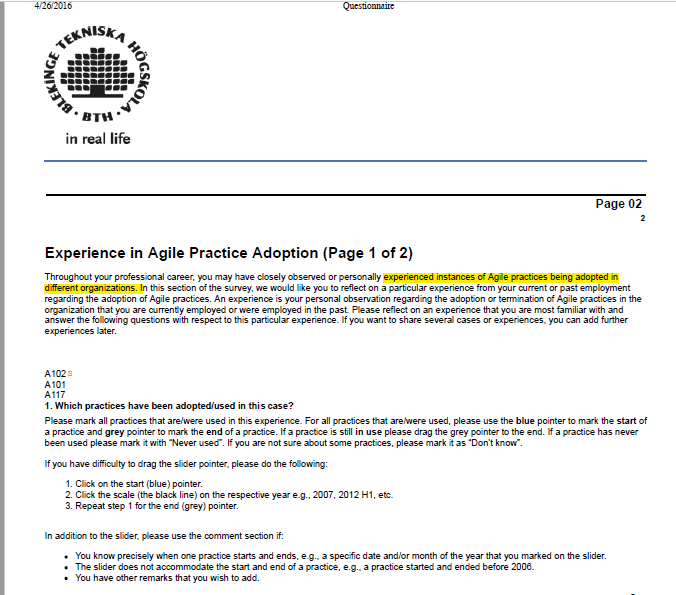
\includegraphics[width=14cm, height=16cm]{Screenshot_1.png}
\end{figure}
\begin{figure}[h]
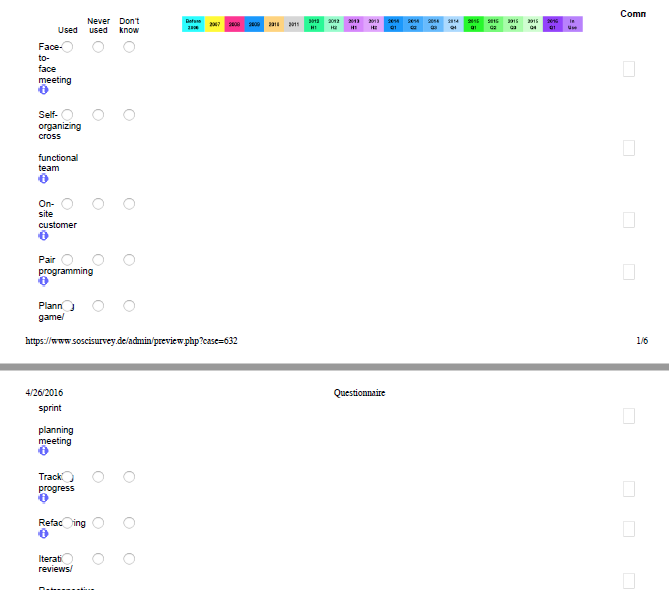
\includegraphics [width=14cm, height=16cm]{Screenshot_2.png}
\end{figure}
\begin{figure}[h]
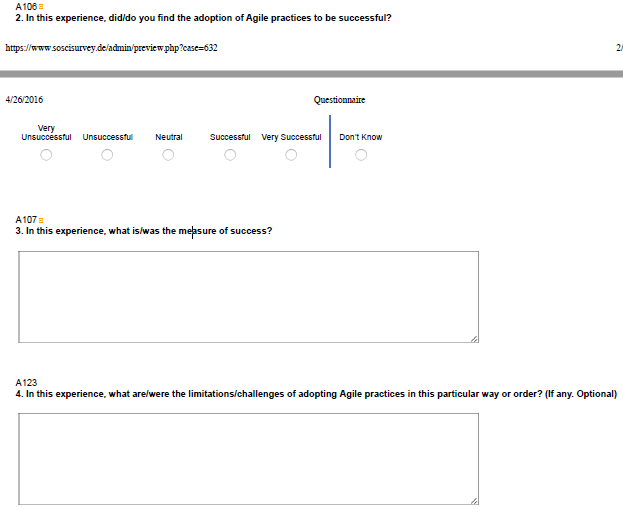
\includegraphics[width=14cm, height=16cm]{Screenshot_3.png}
\end{figure}
\begin{figure}
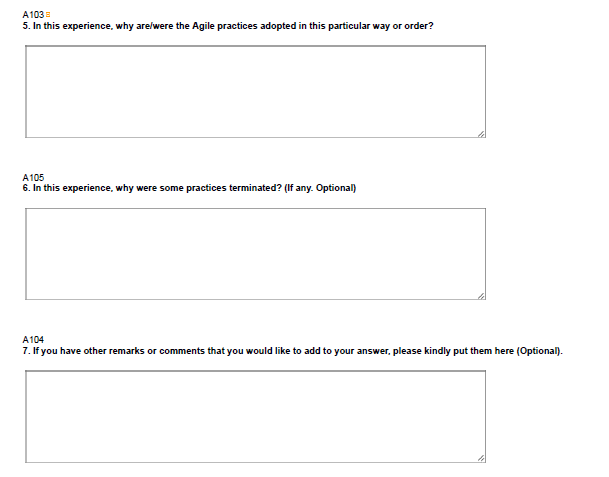
\includegraphics[width=14cm, height=16cm]{Screenshot_4.png}
\end{figure}
\chapter{Invitation letter for participating in interviews} \label{appendix C}
Dear Practitioner,

We are conducting an interview on how Agile practices, e.g., retrospective meetings, pair programming, user stories, and metaphors, etc., can be adopted. This interview is a part of a research project at Blekinge Institute of Technology (BTH). Please kindly find a brief introduction for conducting this interview below.

When adopting an Agile method, e.g., Scrum, eXtreme Programming (XP), etc., usually a number of practices are adopted together. Sometimes you start adopting two or more practices together. Sometimes you start adopting one practice after you master another practice. Which practices should be adopted together? Which practices should be adopted after another? Should a practice be terminated before another can be adopted? Whichever scenario is selected, it might bring different benefits and limitations.

So the goal of this interview is to validate the adoption of Agile practices in particular order. We would like to learn from you as practitioners as you are more aware of implementing the Agile practices. The aim is to understand the benefits and limitations of implementing the Agile practices in our proposed order based on your experience. We would then use your feedback as input for research into how to maximize benefits and minimize limitations of Agile practices adoption. 

Thank you,

In case of any queries regarding the interviews, you can contact:
\begin{flushleft}


Prithvi Raj Sirigudi\\
prsi15@student.bth.se\\
Contact No: +46 76 78 52287\\

Rahul Deekonda\\
rade15@student.bth.se\\
Contact No: +46 767 996 377\\
\end{flushleft}

            \end{appendices}
            
            
\end{document}
